\documentclass[8pt,a4paper]{beamer}
\usepackage{graphicx} % Required for inserting images
\usepackage{color, colortbl}
\usepackage[utf8]{inputenc}
\usepackage[english,serbian]{babel}
\usepackage{indentfirst}
\usepackage{verbatim}
\usepackage[T2A]{fontenc}

\usetheme{Szeged}
\usecolortheme{seahorse}

\title{Informacioni sistem za veterinarsku kliniku "PetCare"}
\author{Alma Hodžić, Milica Nikolić, Mina Ristić}
\institute{Informacioni sistemi \\ Matematički fakultet \\ Univerzitet u Beogradu}
\date{\today} 


\begin{document}

\begin{frame}
\titlepage

\begin{figure}[h!]
    \centering
    \begin{flushleft}
    
\includegraphics[width=15mm]{slika1.jpg}
    \end{flushleft}
\end{figure}
\end{frame}

\begin{frame}{Sadržaj}
\tableofcontents
\end{frame}

\section{Uvod}

\begin{frame}{Uvod}
\begin{itemize}
    \item Veterinarske klinike se u savremenom poslovanju suočavaju sa potrebom za efikasnim upravljanjem podacima, terminima i medicinskom dokumentacijom. \pause
    \item Uvođenje informacionog sistema omogućava unapređenje organizacije rada, smanjenje administrativnih grešaka i poboljšanje kvaliteta usluge. \pause
    \item U okviru ovog projekta predstavljen je informacioni sistem namenjen podršci osnovnim poslovnim procesima veterinarske klinike.

\end{itemize}
\end{frame}
    
\begin{frame}{Uvod}
\begin{itemize}
    \item Informacioni sistem veterinarske klinike \pause
    \begin{itemize}
        \item prati pacijente (životinje) od prijema do završetka terapije \pause
        \item uključuje evidenciju vlasnika, pregleda, terapija i vakcinacija \pause
        \item uključuje evidenciju zaposlenih (veterinar, administrativni radnik, menadžer) \pause
        \item uključuje evidenciju zaliha u magacinu \pause
    \end{itemize}
    \item Zaposleni imaju određene uloge u procesu evidencije, dijagnostike, lečenja i vođenju magacina. \pause
    \item Primarni cilj - unapređenje načina funkcionisanja postojećih sistema u veterinarskoj klinici. \pause
    \item Uvode se online zakazivanje, elektronski kartoni i elektronsko vođenje zaliha.
\end{itemize}
\end{frame}

\section{Analiza sistema}
\subsection{Akteri}
\begin{frame}{Akteri}
\begin{figure}[h!]
        \begin{center}
          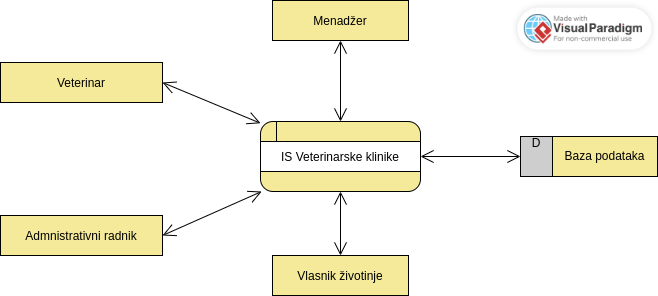
\includegraphics[scale = 0.5]{Dijagrami/dijagram_konteksta.png}
        \end{center}
       \caption{Dijagram konteksta}
    \end{figure}   
\end{frame}


\section{Slučajevi upotrebe}
\begin{frame}{Slučajevi upotrebe}
\vspace{\baselineskip}
\begin{itemize}
	\item Razlikujemo 3 glavna slučaja upotrebe: \pause
    \begin{itemize}
        \item Upravljanje terminima i zakazivanje pregleda \pause
        \item Evidencija pregleda i tretmana životinja \pause
        \item Upravljanje zalihama lekova i jednokratne opreme \pause
    \end{itemize}
    \item Svaki od njih je podeljen na više manjih slučajeva.
    
\end{itemize}
\end{frame}

\subsection{Upravljanje terminima i zakazivanje pregleda}
\begin{frame}{Upravljanje terminima i zakazivanje pregleda}
        \begin{figure}[h!]
        \begin{center}
          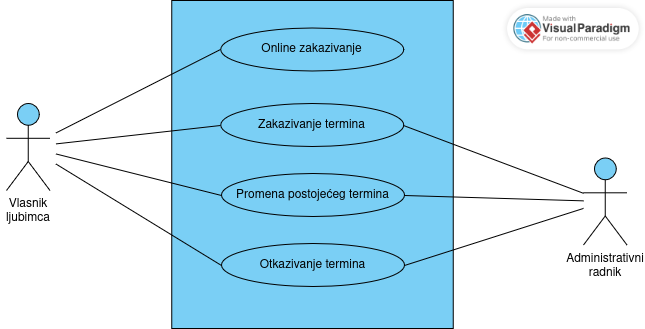
\includegraphics[scale = 0.5]{Dijagrami/dijagramSlu.png}
        \end{center}
       \caption{Dijagram slučaja upotrebe}
    \end{figure}   
\end{frame}

\begin{frame}{Online zakazivanje}
        \begin{figure}[h!]
        \begin{center}
          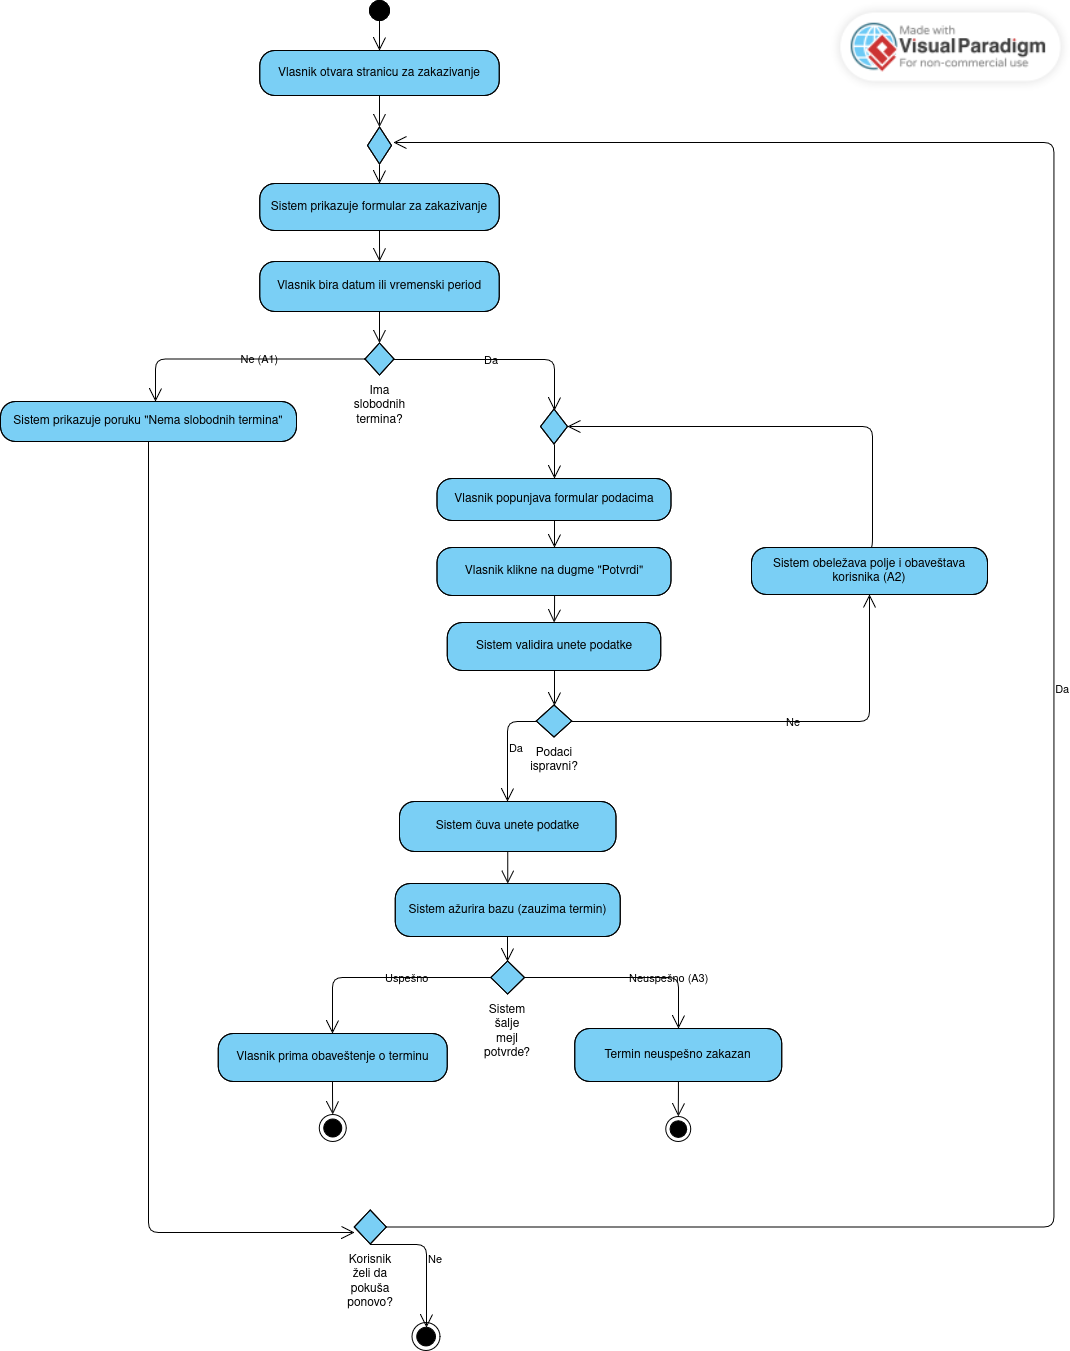
\includegraphics[scale = 0.15]{Dijagrami/dijagramAktivnosti1.png}
        \end{center}
       \caption{Dijagram aktivnosti}
    \end{figure}   
\end{frame}

\begin{frame}{Zakazivanje termina}
        \begin{figure}[h!]
        \begin{center}
          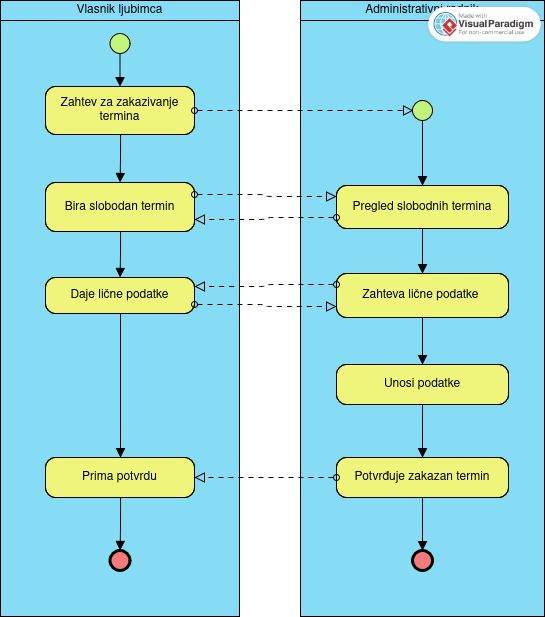
\includegraphics[scale = 0.3]{Dijagrami/bpmnZT.png}
        \end{center}
       \caption{BPMN dijagram}
    \end{figure}   
\end{frame}

\begin{frame}{Zakazivanje termina}
        \begin{figure}[h!]
        \begin{center}
          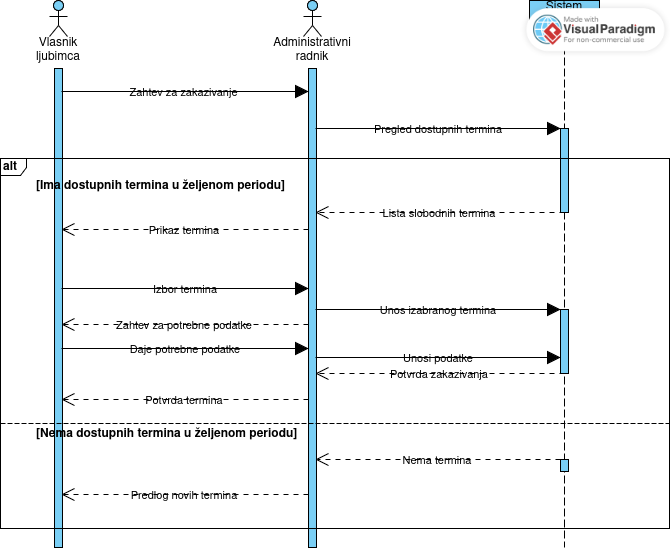
\includegraphics[scale = 0.3]{Dijagrami/dijagramSekvenceZP.png}
        \end{center}
       \caption{Dijagram sekvence}
    \end{figure}   
\end{frame}


\subsection{Evidencija pregleda i tretmana životinja}

\begin{frame}{Upravljanje zalihama lekova i jednokratne opreme}
        \begin{figure}[h!]
        \begin{center}
          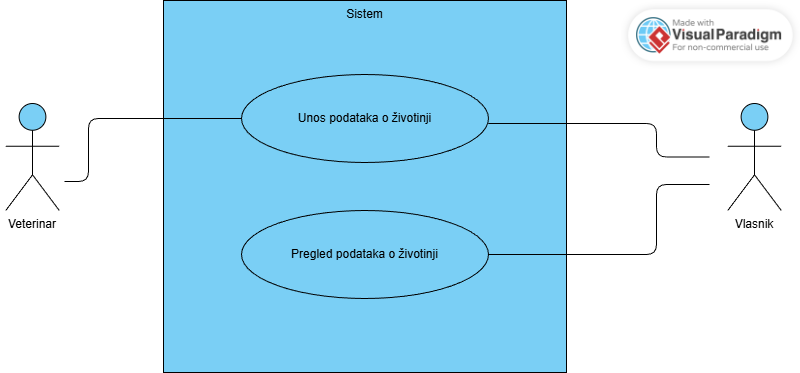
\includegraphics[scale = 0.5]{SlucajeviUpotrebe/su2.png}
        \end{center}
       \caption{Dijagram slučaja upotrebe}
    \end{figure}   
\end{frame}

        \begin{figure}[h!]
        \begin{center}
          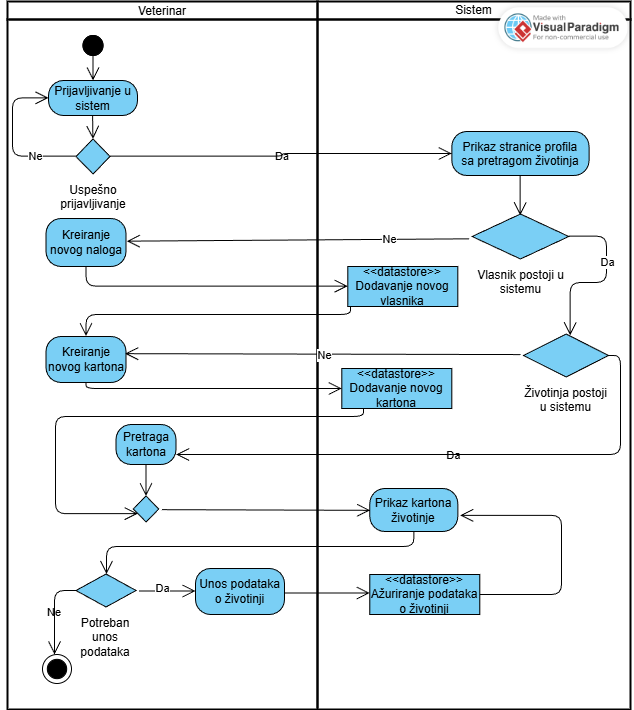
\includegraphics[scale = 0.5]{Dijagrami/dijagram_aktivnosti_unos_podataka.png}
        \end{center}
       \caption{Unos podataka - Dijagram aktivnosti}
    \end{figure}   

        \begin{figure}[h!]
        \begin{center}
          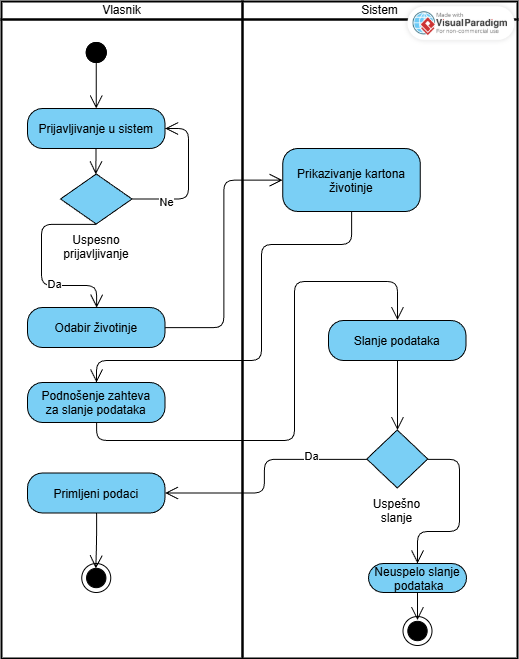
\includegraphics[scale = 0.5]{Dijagrami/dijagram_aktivnosti_pregled_podataka.png}
        \end{center}
       \caption{Pregled podataka - Dijagram aktivnosti}
    \end{figure}   




\subsection{Upravljanje zalihama lekova i jednokratne opreme}

\begin{frame}{Upravljanje zalihama lekova i jednokratne opreme}
        \begin{figure}[h!]
        \begin{center}
          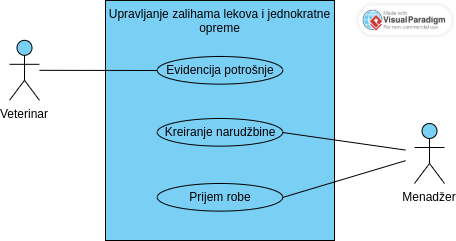
\includegraphics[scale = 0.5]{Dijagrami/dijagram_slucajeva_upotrebe_3.png}
        \end{center}
       \caption{Dijagram slučaja upotrebe}
    \end{figure}   
\end{frame}

\begin{frame}{Evidencija potrošnje}
        \begin{figure}[h!]
        \begin{center}
          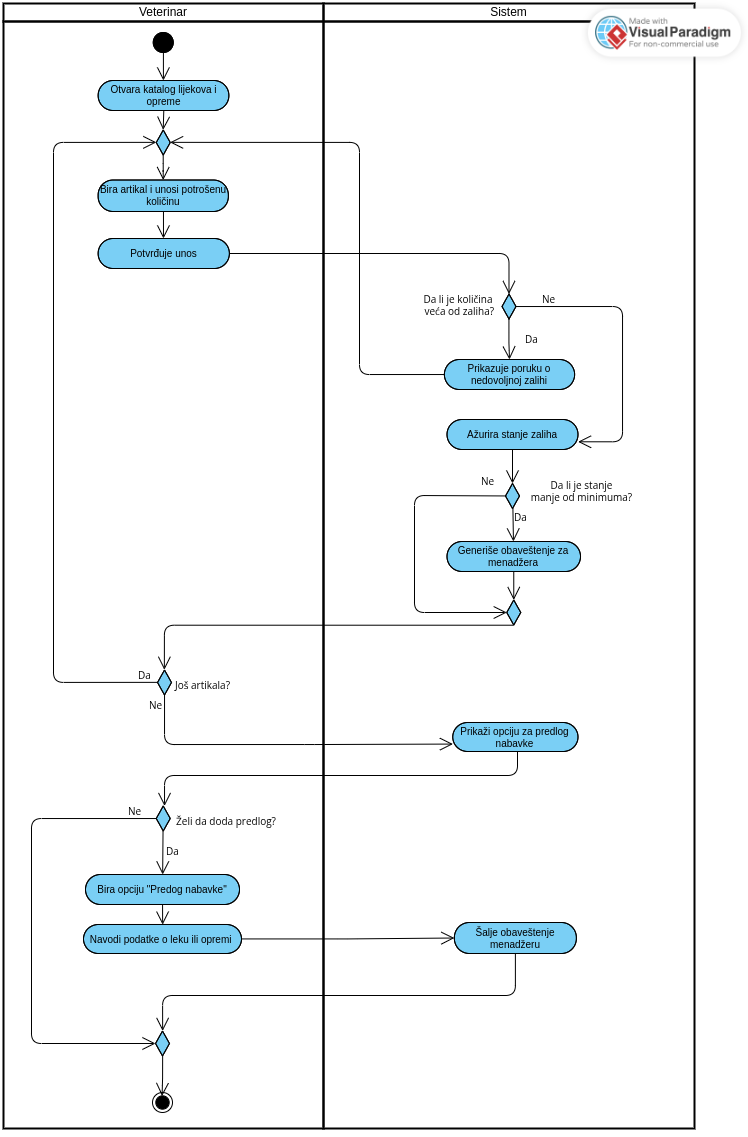
\includegraphics[scale = 0.15]{Dijagrami/dijagram_aktivnosti_evidencija_potrosnje.png}
        \end{center}
       \caption{Dijagram aktivnosti}
    \end{figure}   
\end{frame}

\begin{frame}{Kreiranje narudžbine}
        \begin{figure}[h!]
        \begin{center}
          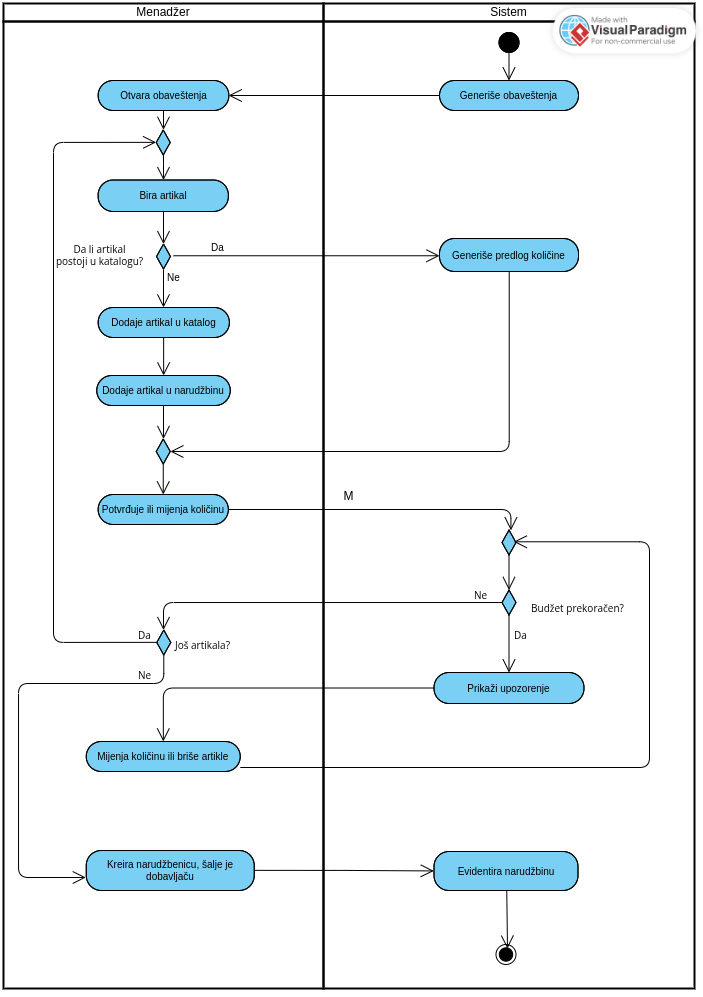
\includegraphics[scale = 0.2]{Dijagrami/dijagram_aktivnosti_kreiranje_narudzbine.png}
        \end{center}
       \caption{Dijagram aktivnosti}
    \end{figure}   
\end{frame}

\begin{frame}{Prijem robe}
        \begin{figure}[h!]
        \begin{center}
          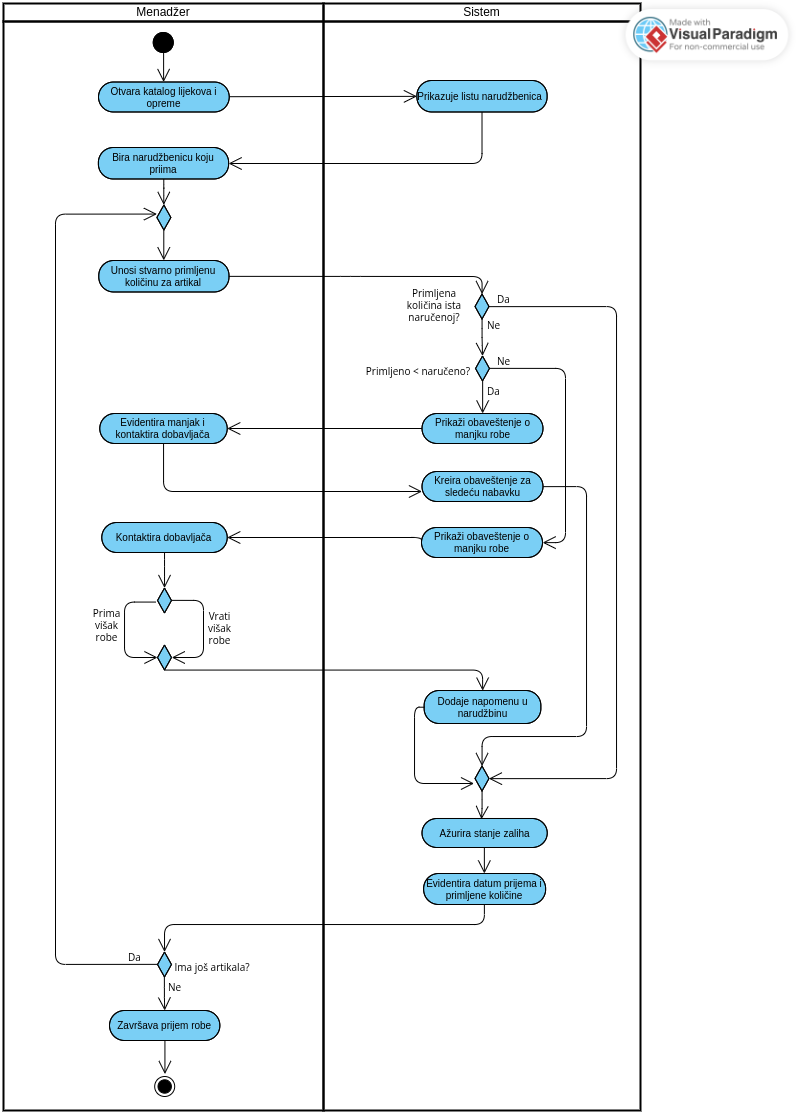
\includegraphics[scale = 0.15]{Dijagrami/dijagram_aktivnosti_prijem_robe.png}
        \end{center}
       \caption{Dijagram aktivnosti}
    \end{figure}   
\end{frame}









\section{Opis baze podataka}

\begin{frame}{Model baze podataka}
        \begin{figure}[h!]
        \begin{center}
          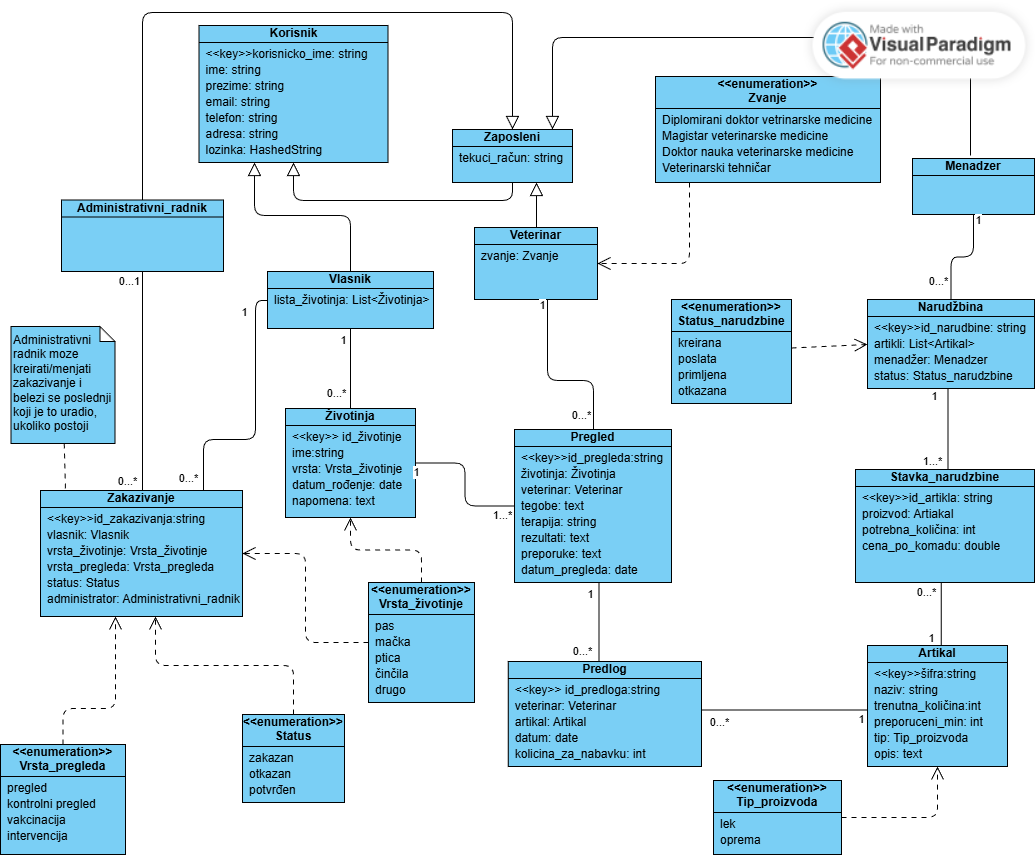
\includegraphics[scale = 0.2]{Dijagrami/dijagram_klasa.png}
        \end{center}
    \end{figure}   
\end{frame}











\section{Arhitektura sistema}
\begin{frame}{Odabir arhitekture}
\vspace{\baselineskip}
\begin{itemize}
	\item Arhitektura je odabrana tako da ispuni što je više moguće sledeće zahteve: \pause
    \begin{itemize}
        \item Bezbednost sistema \pause
        \item Lakoća korišćenja \pause
        \item Dostupnost \pause
        \item Pouzdanost
    \end{itemize}
\end{itemize}
\end{frame}

\begin{frame}{Dijagram arhitekture}
        \begin{figure}[h!]
        \begin{center}
          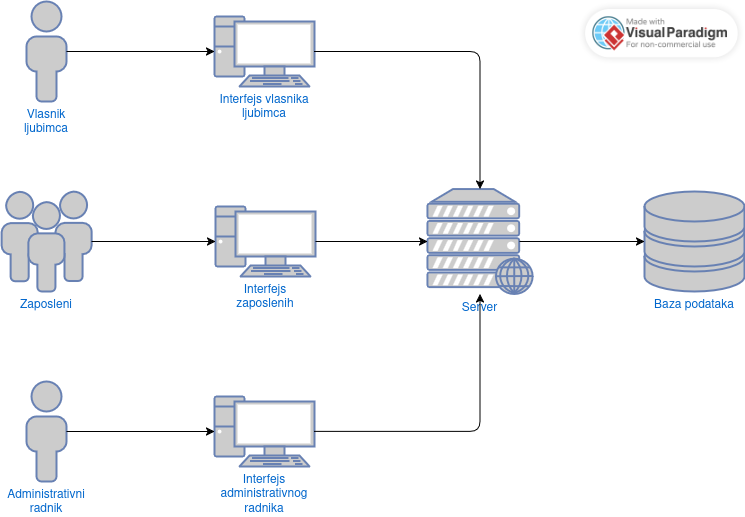
\includegraphics[scale = 0.3]{Dijagrami/arhitektura.png}
        \end{center}
    \end{figure}   
\end{frame}

\begin{frame}{Komponente arhitekture}
        \begin{figure}[h!]
        \begin{center}
          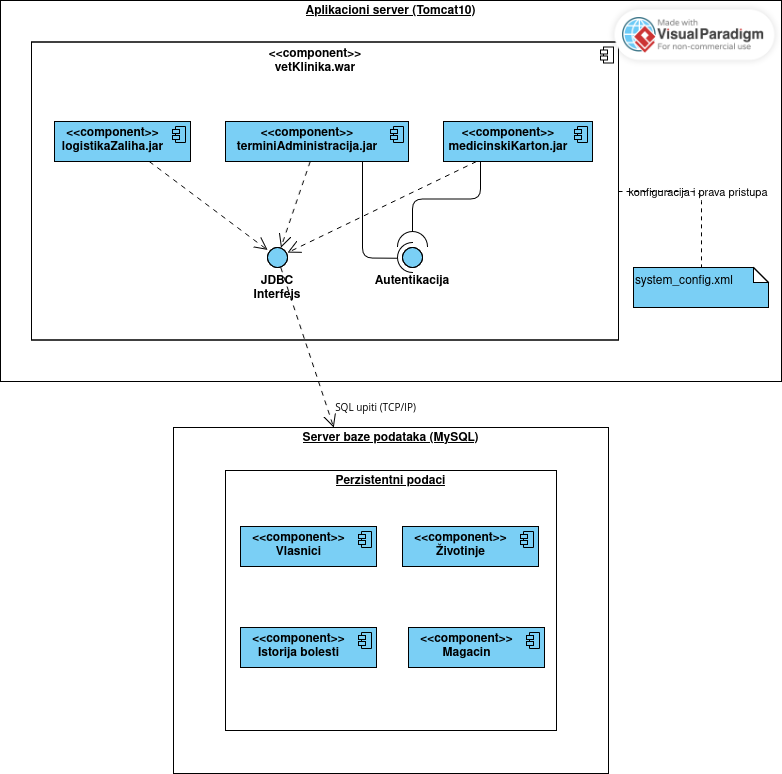
\includegraphics[scale = 0.24]{Dijagrami/arhitekturaDijagram.png}
        \end{center}
       \caption{Dijagram komponenti}
    \end{figure}   
\end{frame}

\section{Korisnički interfejs}
\begin{frame}{Online zakazivanje}
        \begin{figure}[h!]
        \begin{center}
          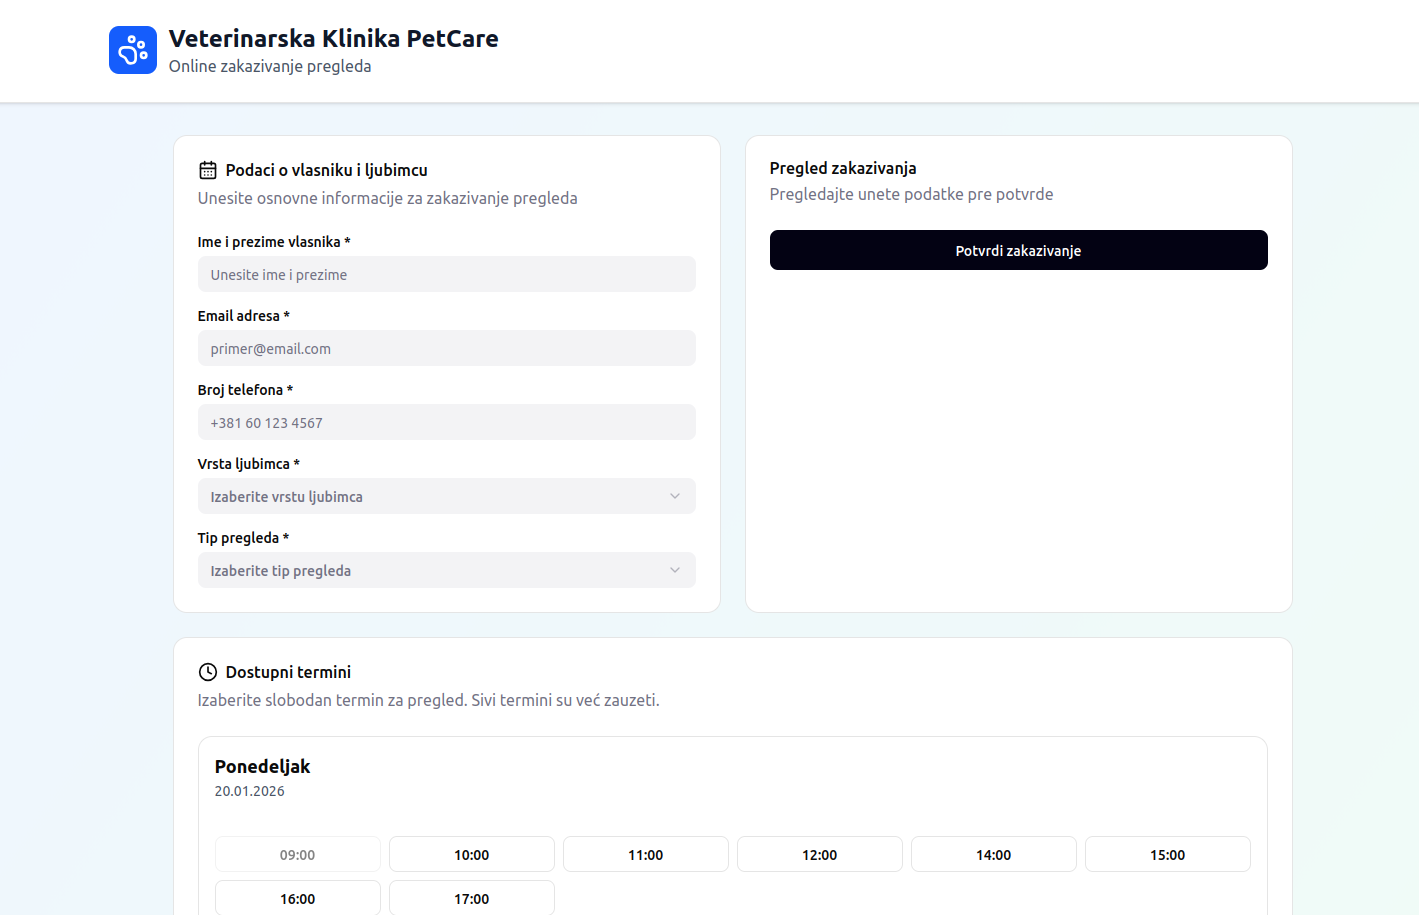
\includegraphics[scale = 0.18]{UI/online_zakazivanje1.png}
        \end{center}
    \end{figure}   
\end{frame}

\begin{frame}{Online zakazivanje}
        \begin{figure}[h!]
        \begin{center}
          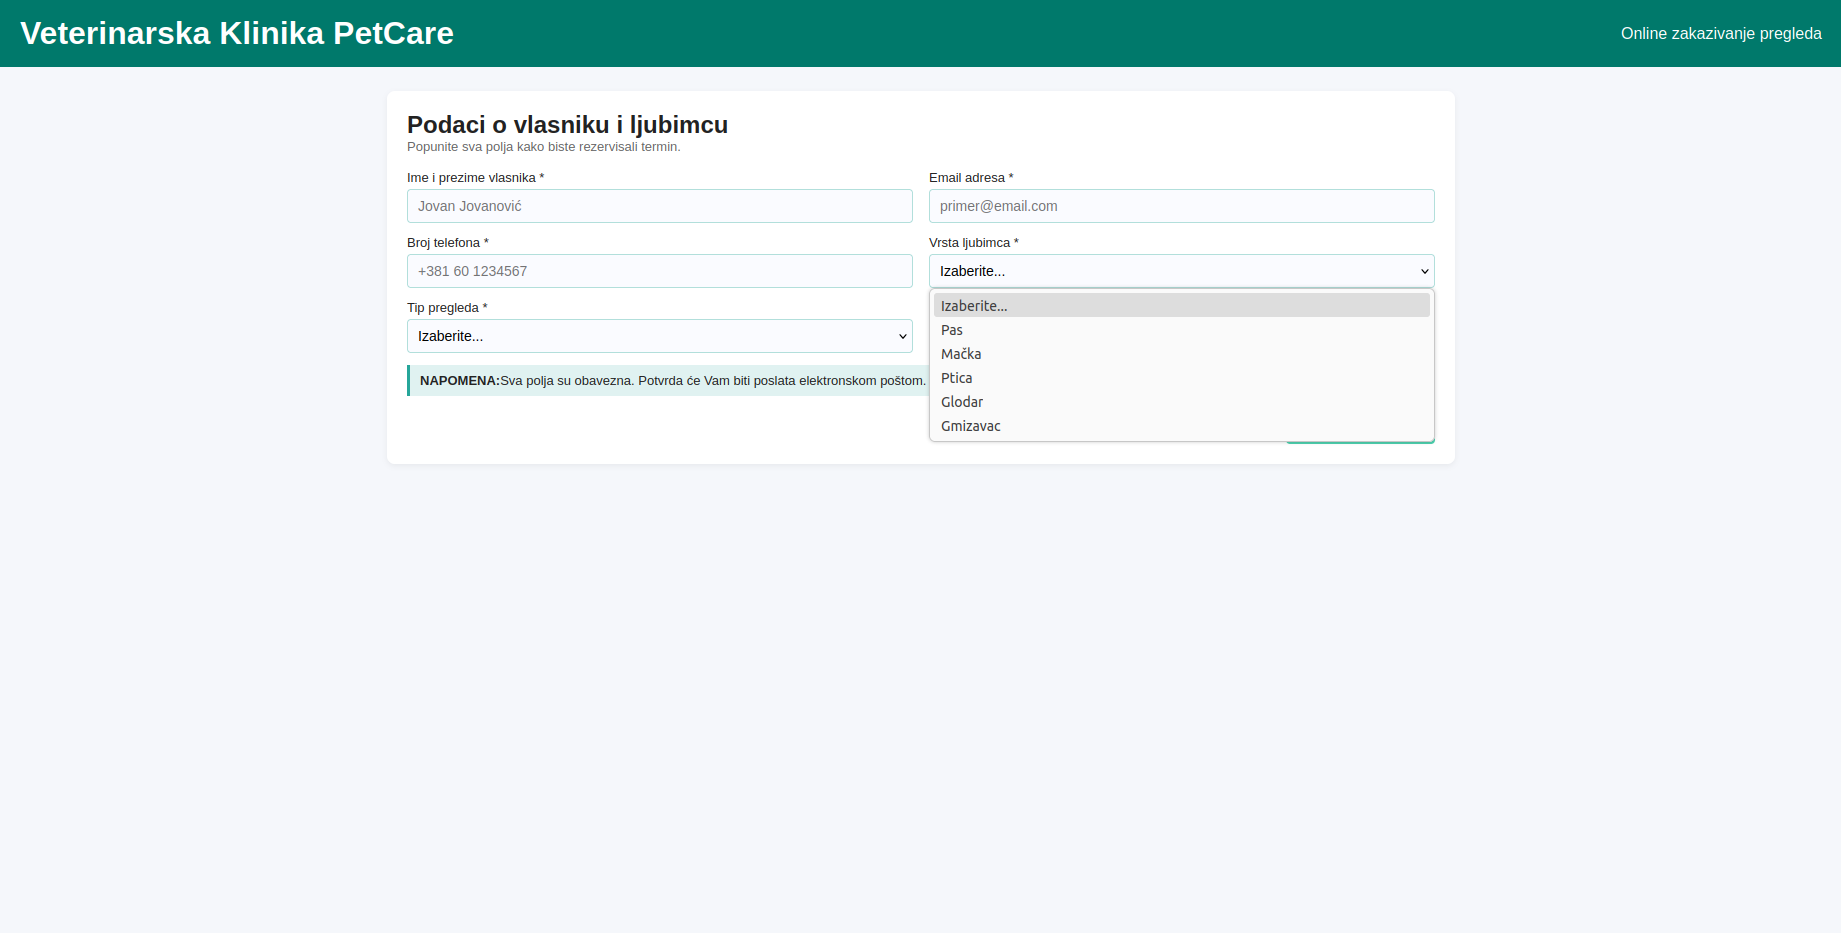
\includegraphics[scale = 0.18]{UI/online_zakazivanje2.png}
        \end{center}
    \end{figure}   
\end{frame}

\begin{frame}{Online zakazivanje}
        \begin{figure}[h!]
        \begin{center}
          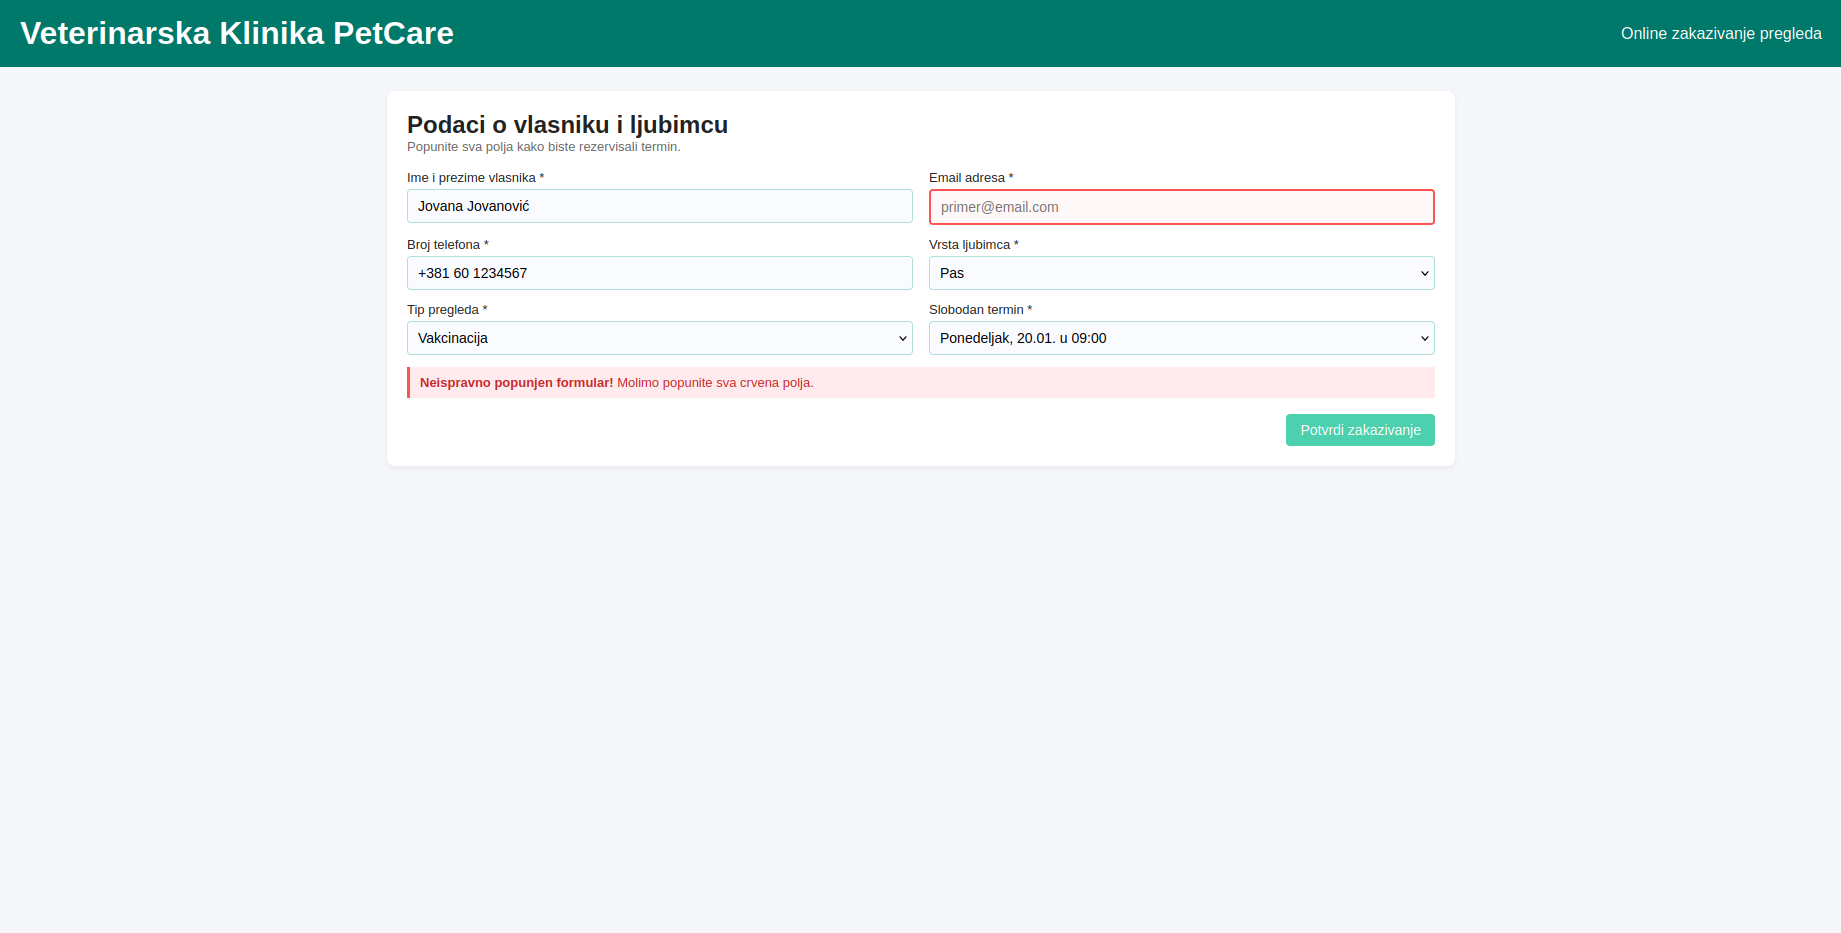
\includegraphics[scale = 0.18]{UI/online_zakazivanje5.png}
        \end{center}
    \end{figure}   
\end{frame}

\begin{frame}{Online zakazivanje}
        \begin{figure}[h!]
        \begin{center}
          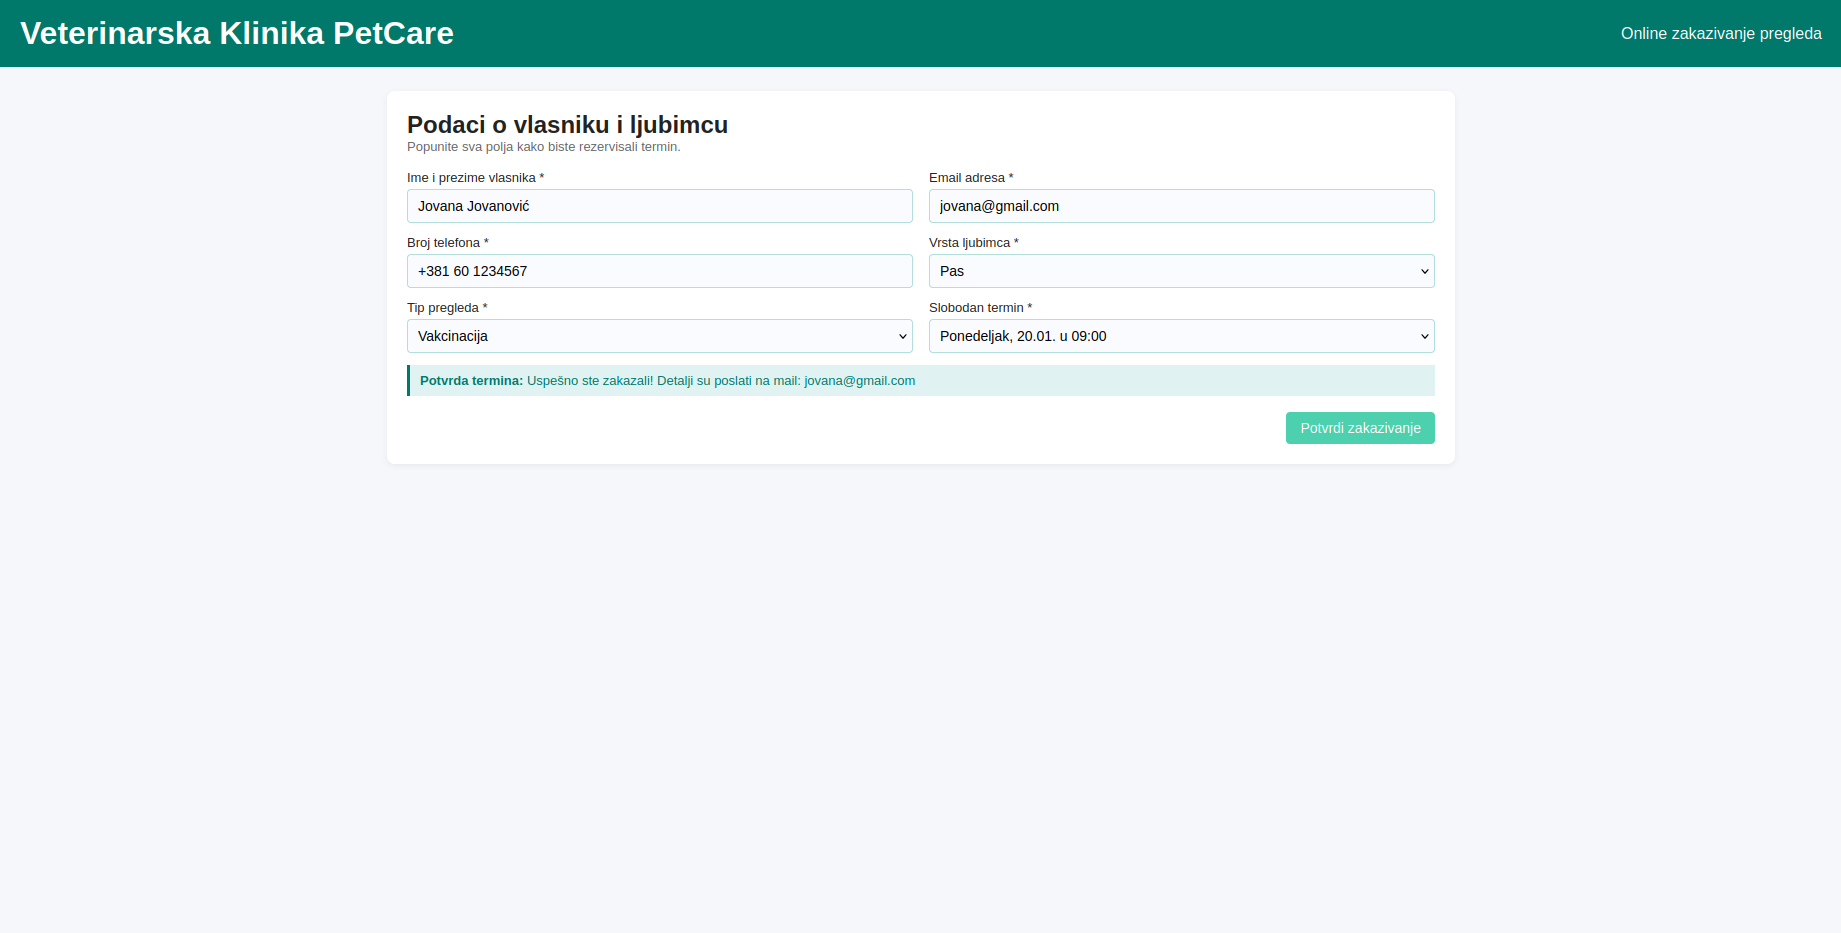
\includegraphics[scale = 0.18]{UI/online_zakazivanje6.png}
        \end{center}
    \end{figure}   
\end{frame}

\begin{frame}{Interfejs administrativnog radnika}
        \begin{figure}[h!]
        \begin{center}
          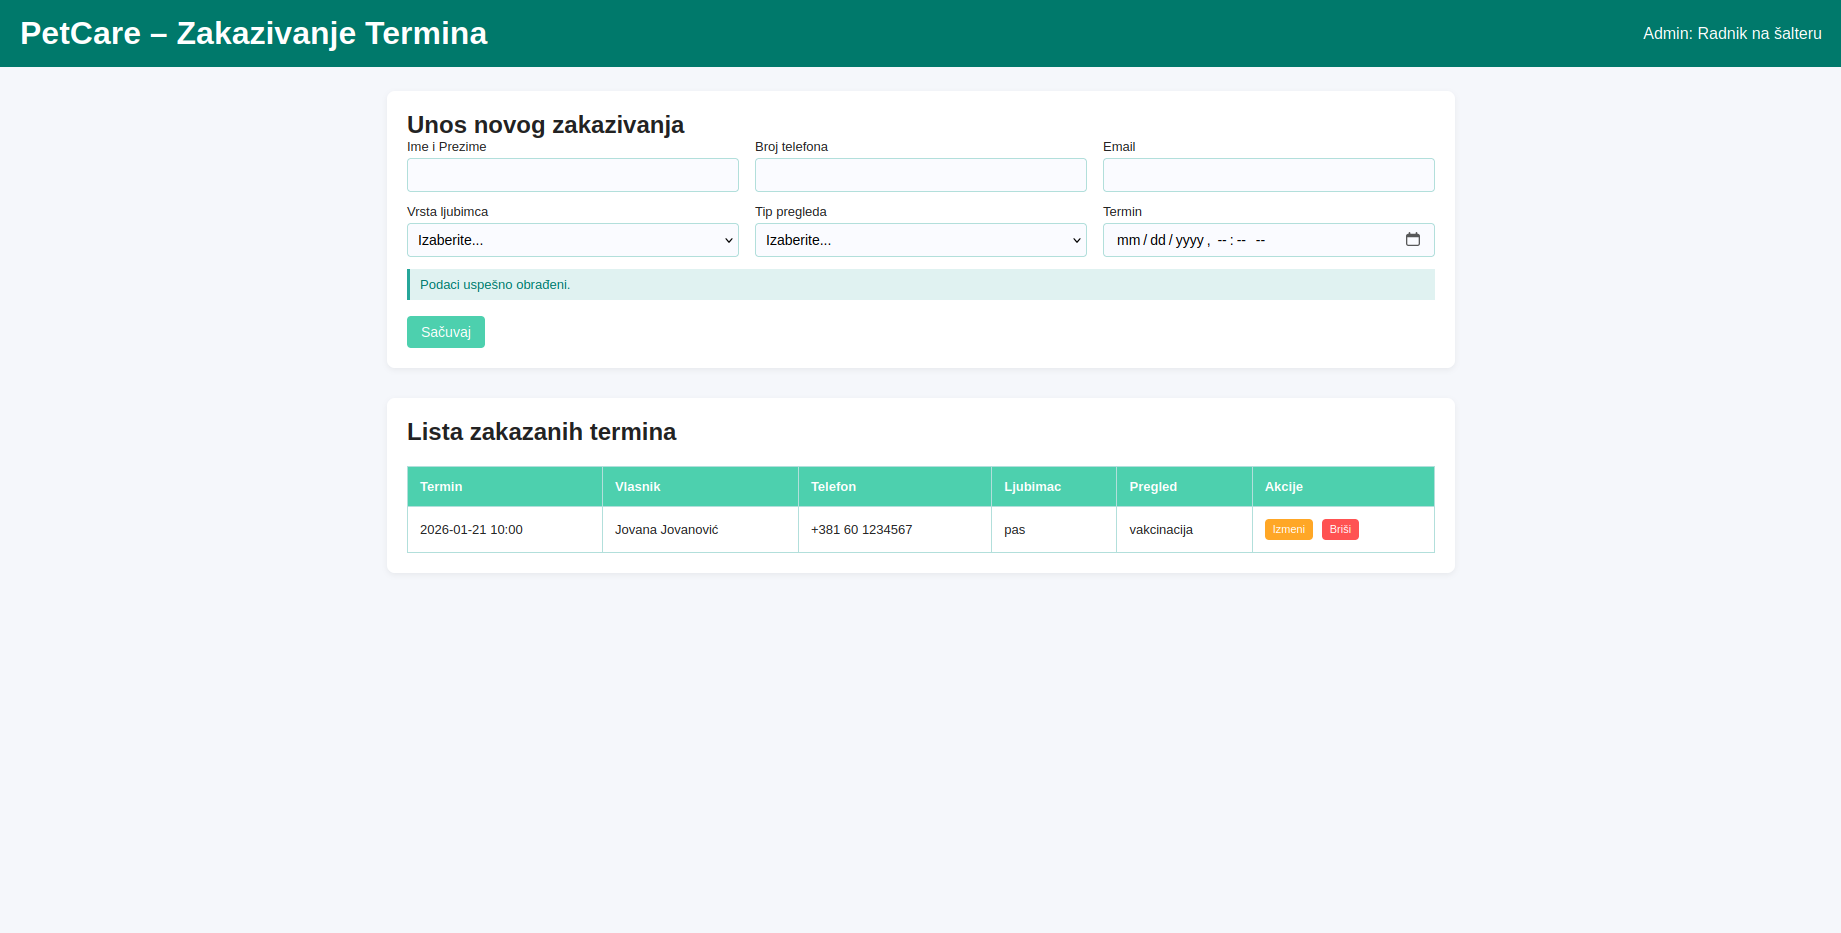
\includegraphics[scale = 0.18]{UI/zakazivanje5.png}
        \end{center}
    \end{figure}   
\end{frame}

\begin{frame}{Evidencija potrošnje}
        \begin{figure}[h!]
        \begin{center}
          
\includegraphics[scale = 0.18]{UI/Evidencija_potrosnje_1.png}
        \end{center}
    \end{figure}   
\end{frame}

\begin{frame}{Evidencija potrošnje}
        \begin{figure}[h!]
        \begin{center}
          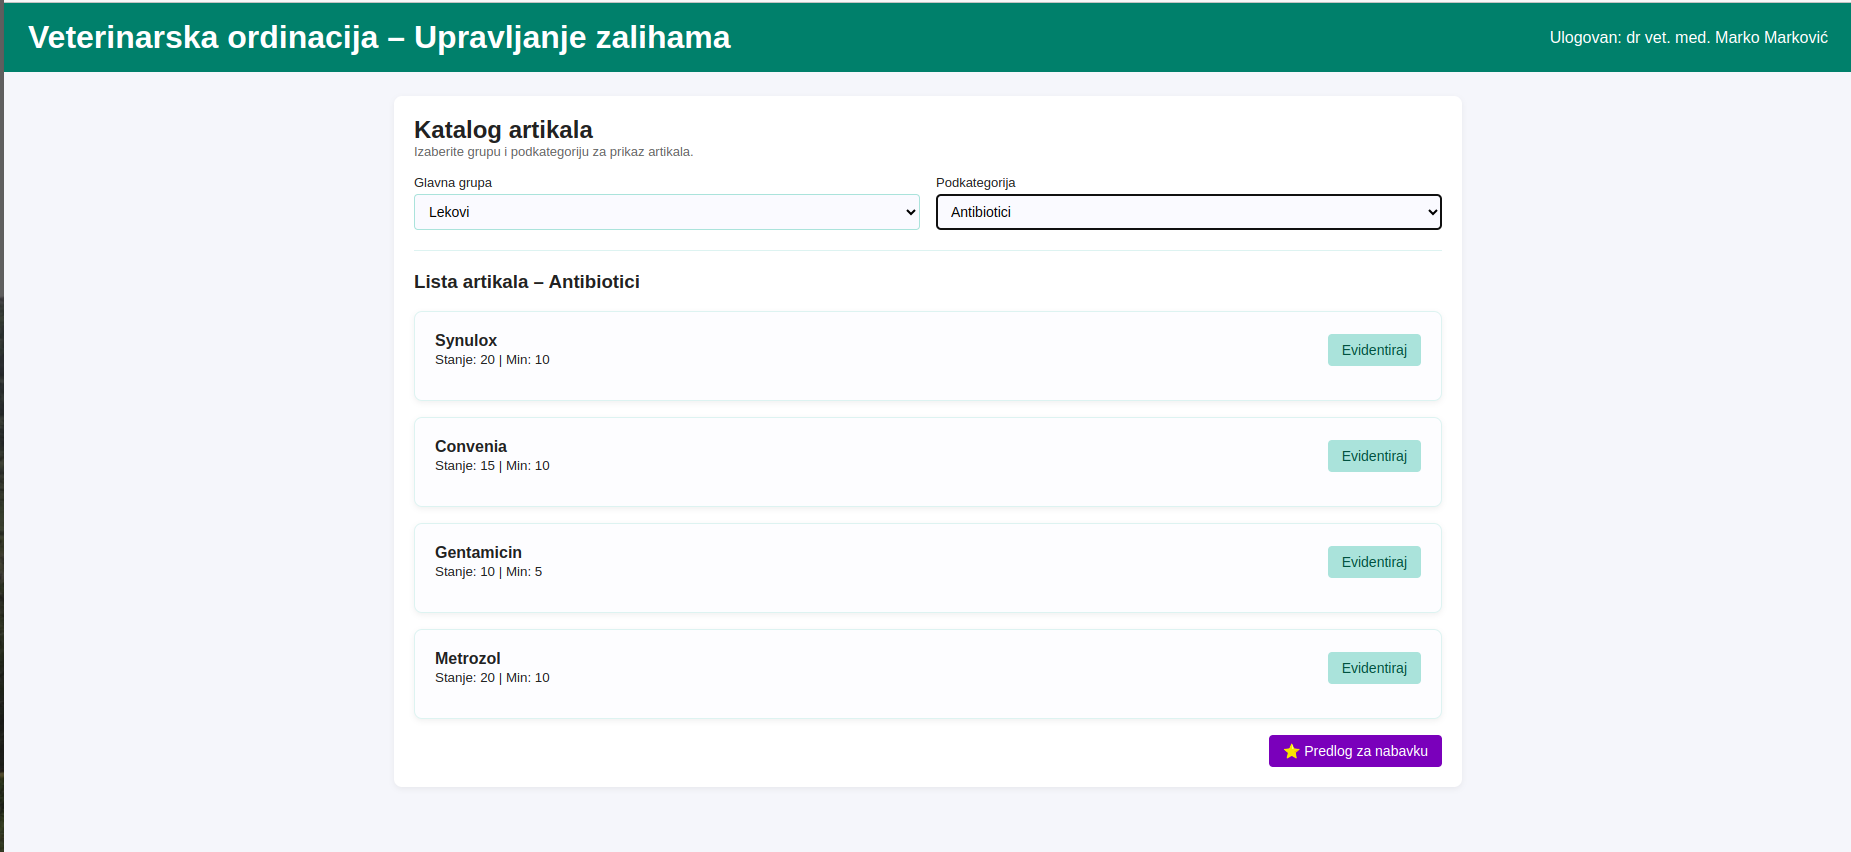
\includegraphics[scale = 0.18]{UI/Evidencija_potrosnje_2.png}
        \end{center}
    \end{figure}   
\end{frame}

\begin{frame}{Evidencija potrošnje}
        \begin{figure}[h!]
        \begin{center}
          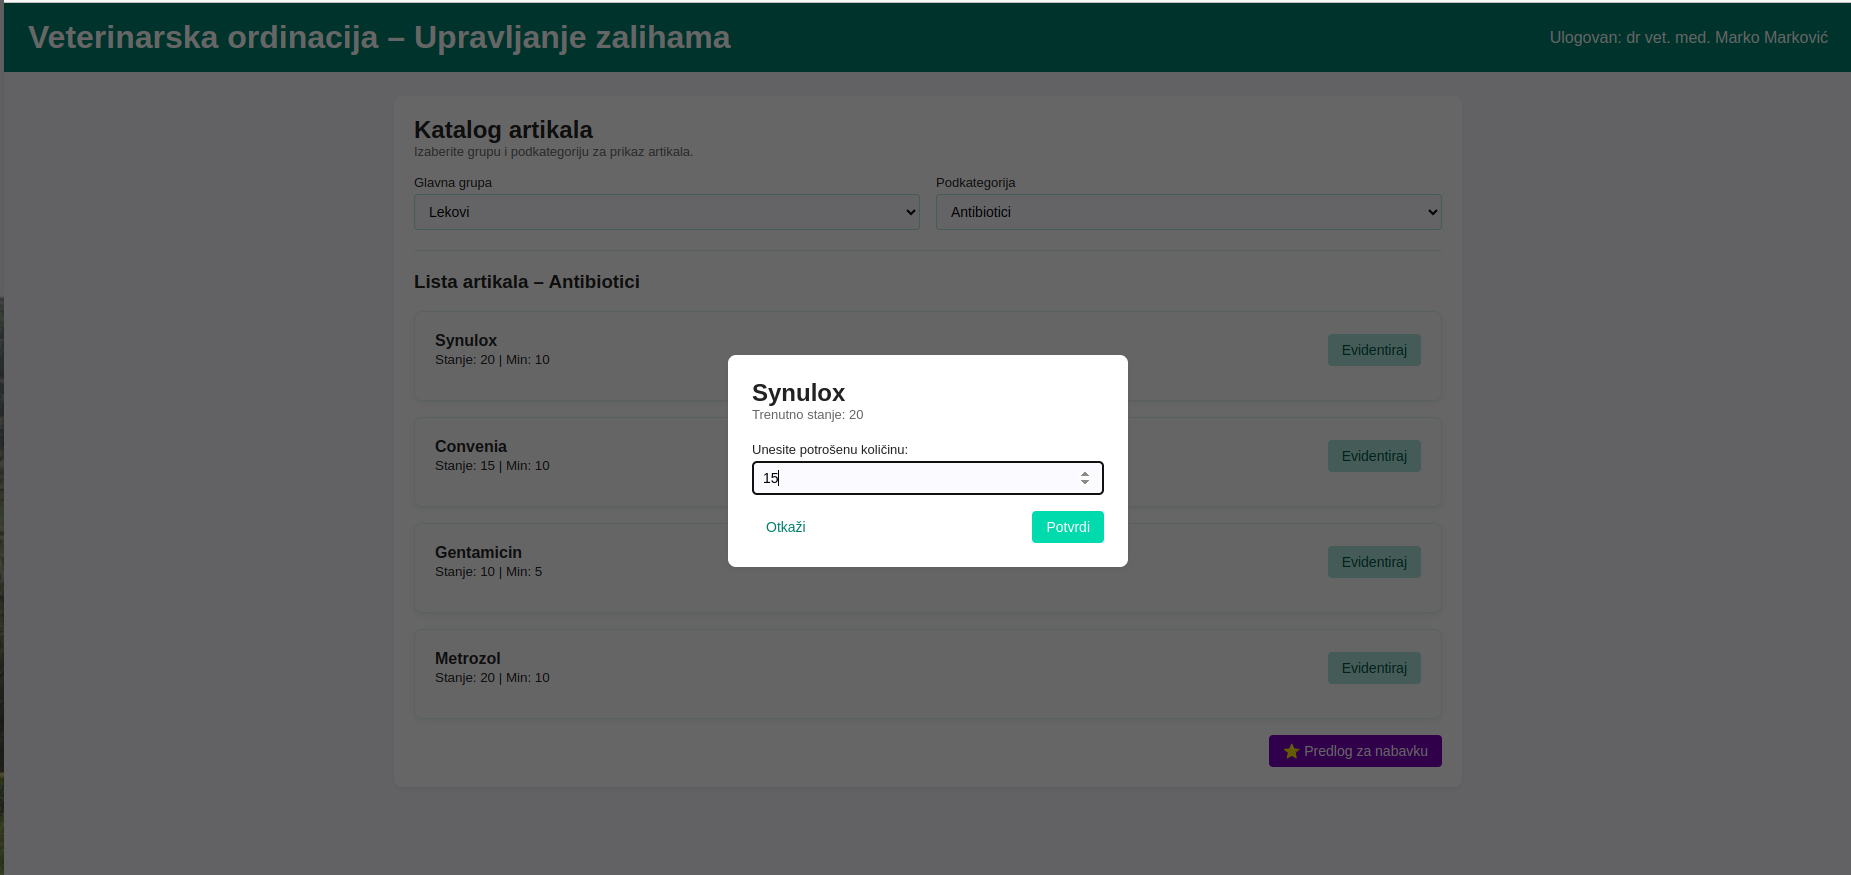
\includegraphics[scale = 0.18]{UI/Evidencija_potrosnje_3.png}
        \end{center}
    \end{figure}   
\end{frame}

\begin{frame}{Evidencija potrošnje}
        \begin{figure}[h!]
        \begin{center}
          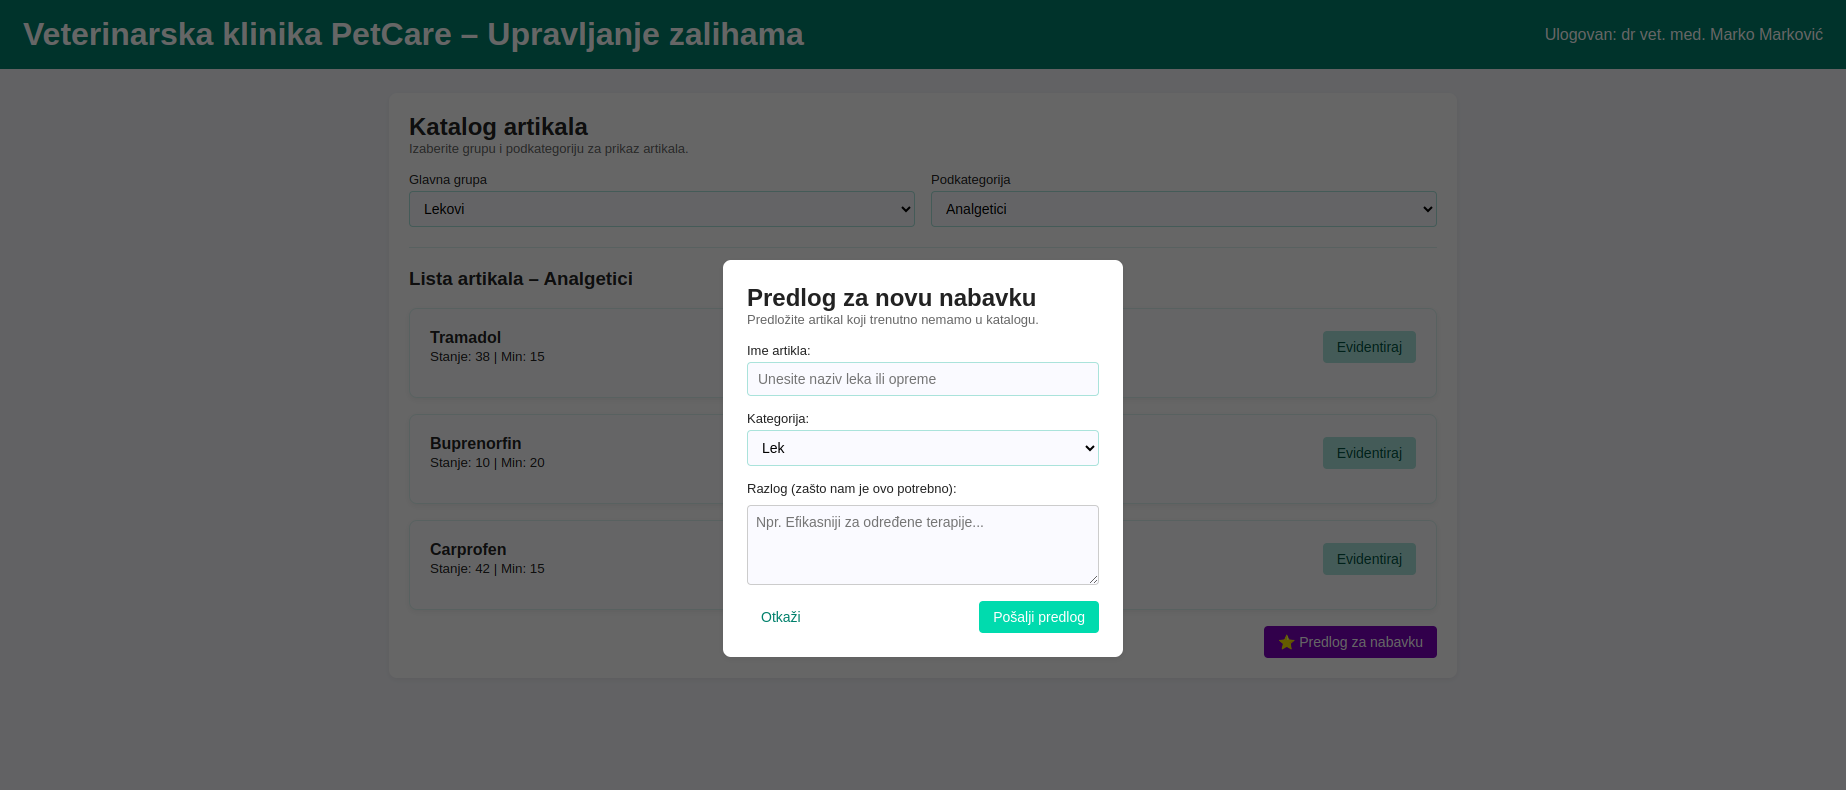
\includegraphics[scale = 0.18]{UI/Evidencija_potrosnje_4.png}
        \end{center}
    \end{figure}   
\end{frame}

\begin{frame}{Narudžbine}
        \begin{figure}[h!]
        \begin{center}
          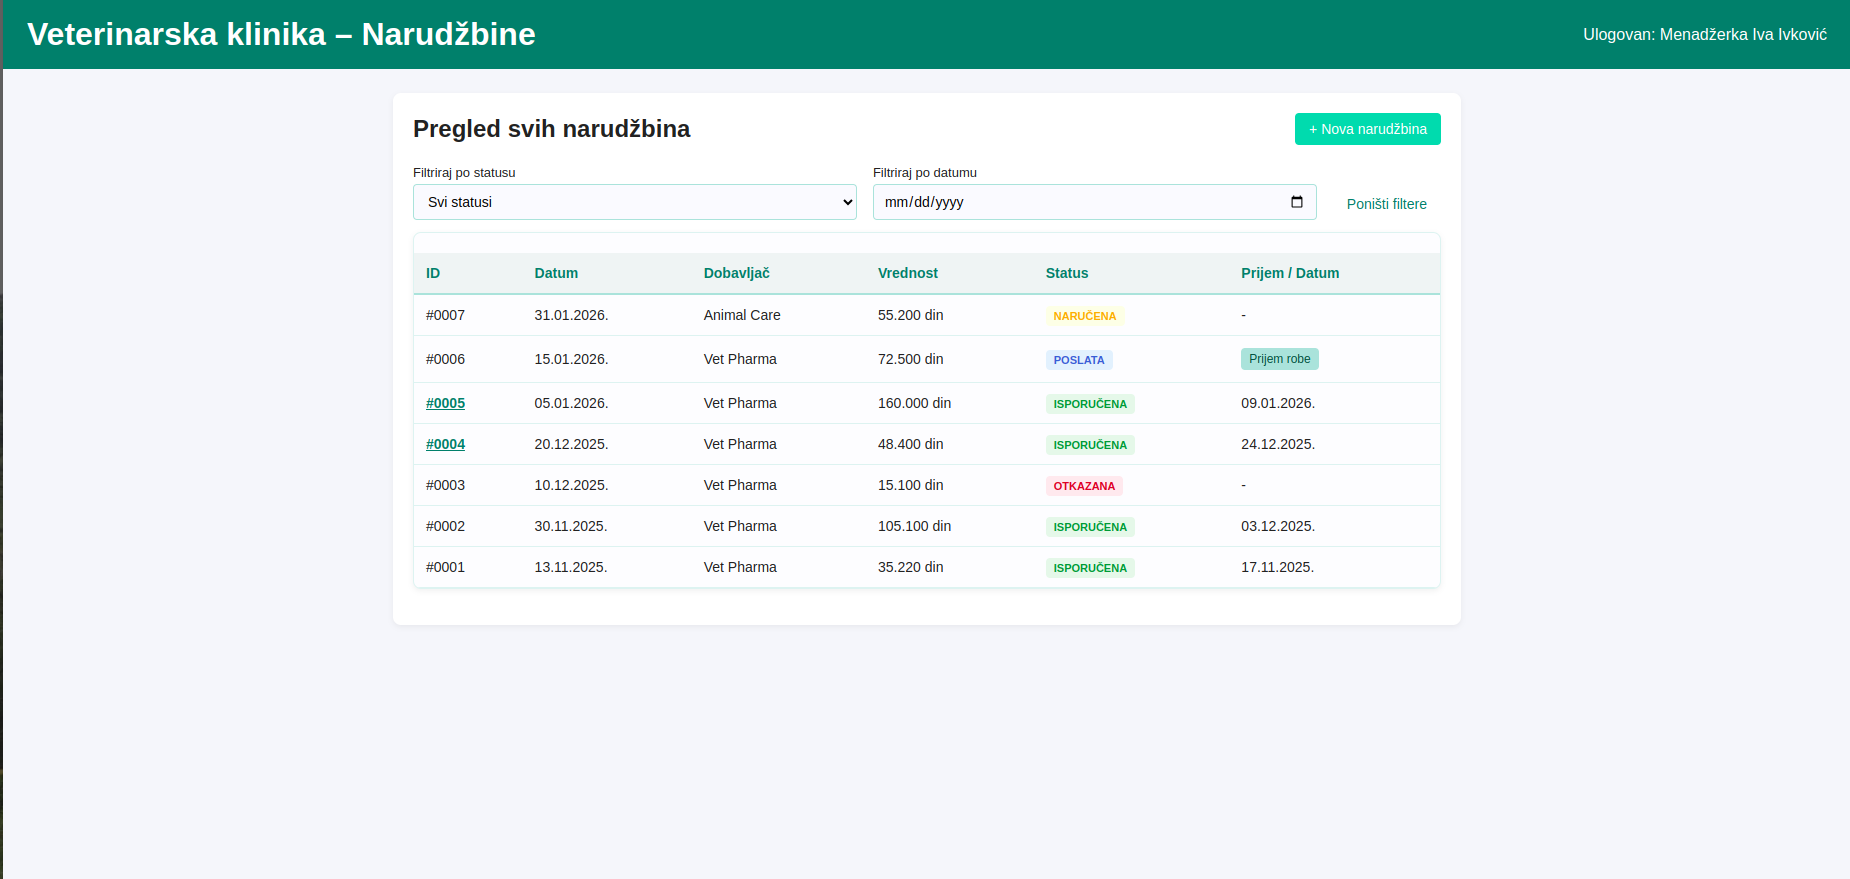
\includegraphics[scale = 0.18]{UI/Narudzbine_1.png}
        \end{center}
    \end{figure}   
\end{frame}

\begin{frame}{Narudžbine}
        \begin{figure}[h!]
        \begin{center}
          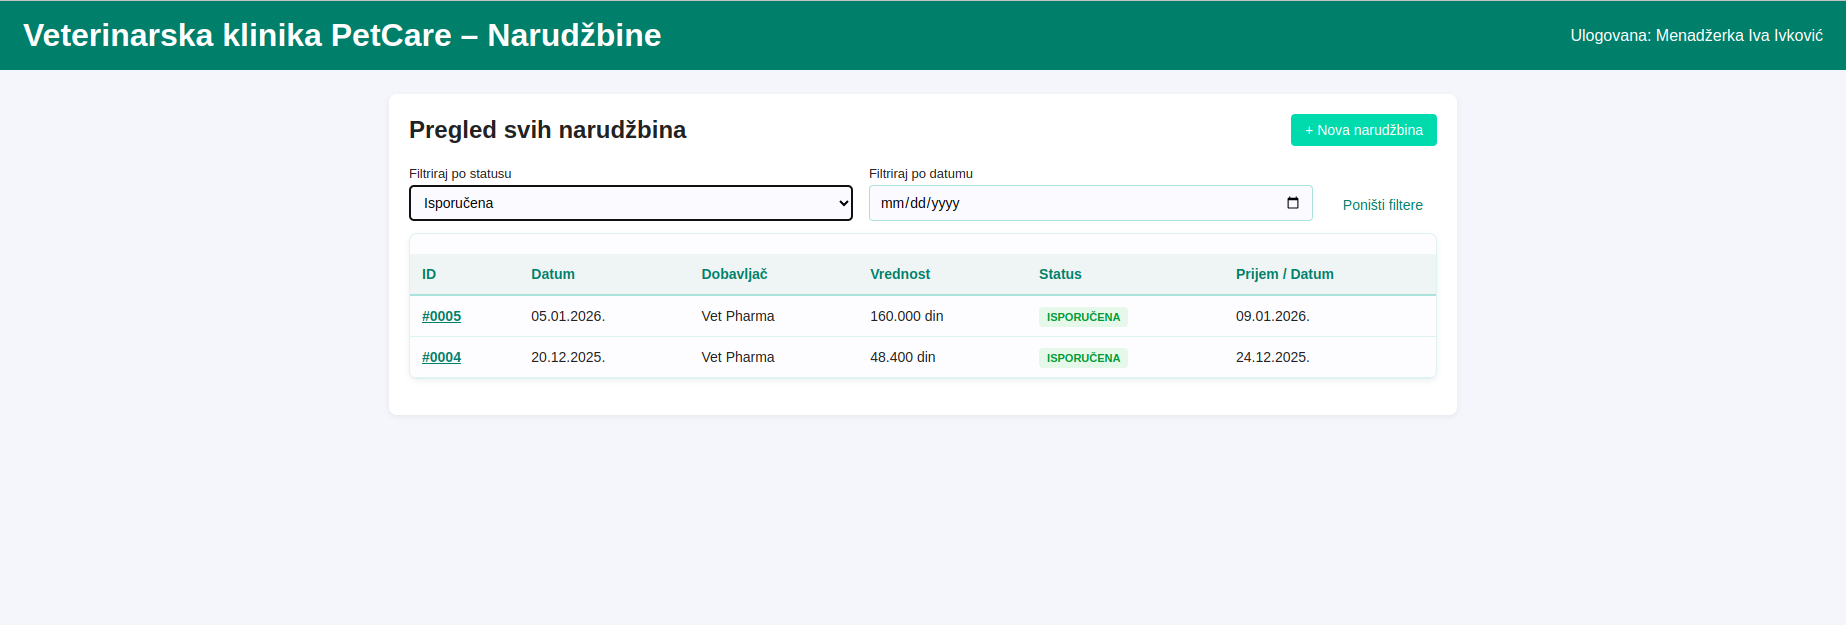
\includegraphics[scale = 0.18]{UI/Narudzbine_2.png}
        \end{center}
    \end{figure}   
\end{frame}

\begin{frame}{Narudžbine}
        \begin{figure}[h!]
        \begin{center}
          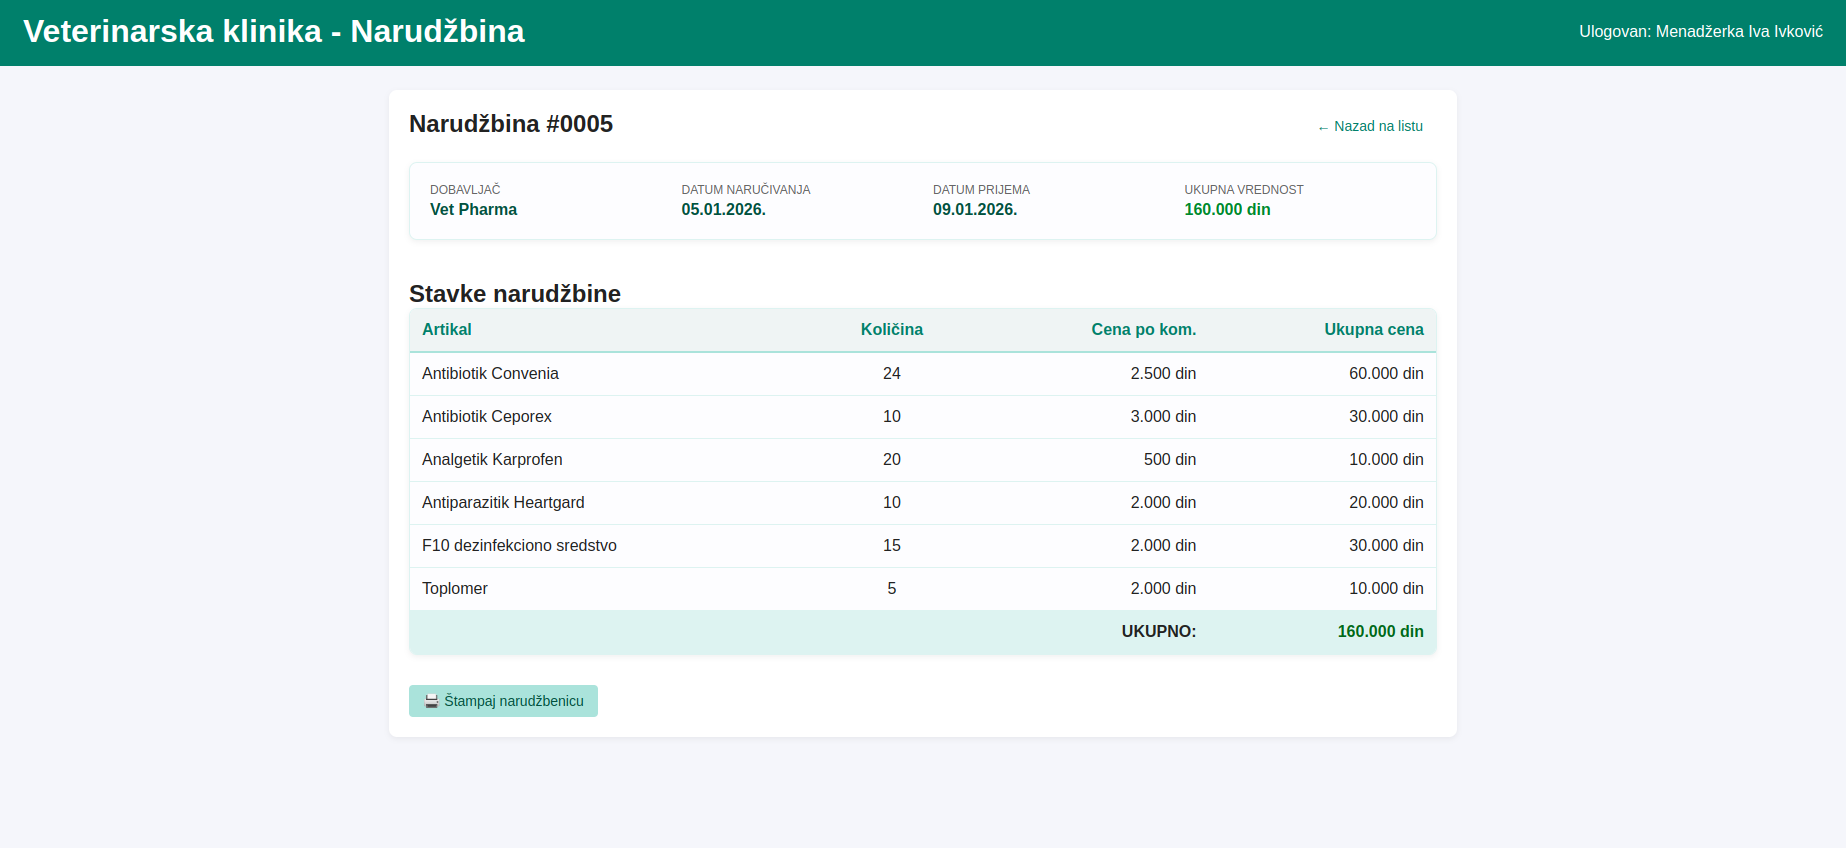
\includegraphics[scale = 0.18]{UI/Narudzbine_3.png}
        \end{center}
    \end{figure}   
\end{frame}


\begin{frame}{Nova narudžbina}
        \begin{figure}[h!]
        \begin{center}
          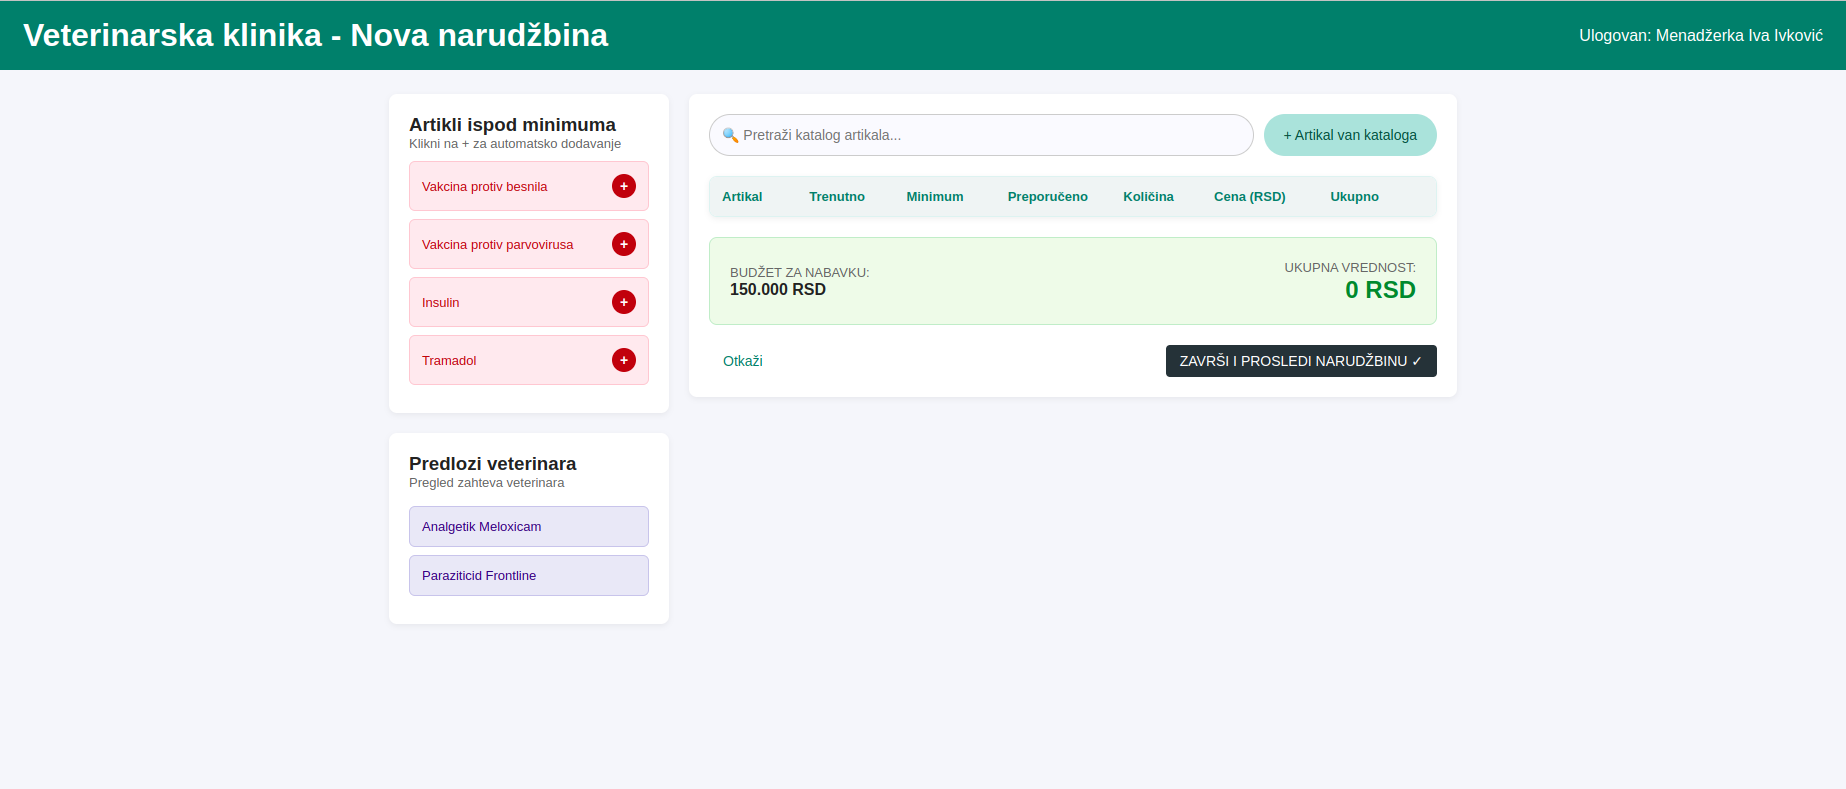
\includegraphics[scale = 0.18]{UI/Nova_narudzbina_1.png}
        \end{center}
    \end{figure}   
\end{frame}

\begin{frame}{Nova narudžbina}
        \begin{figure}[h!]
        \begin{center}
          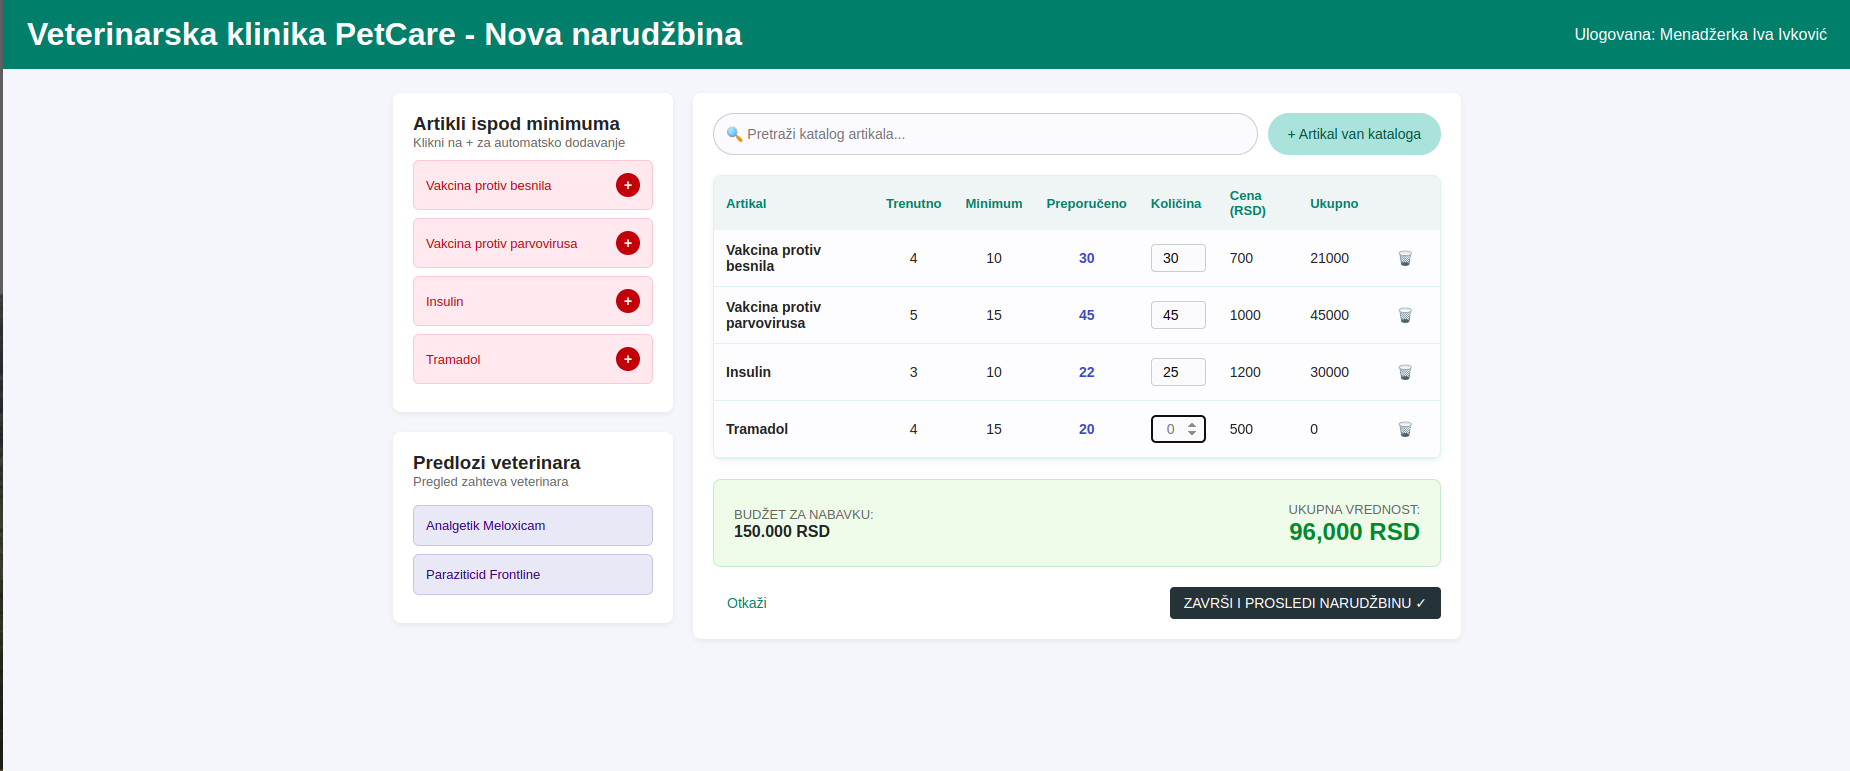
\includegraphics[scale = 0.18]{UI/Nova_narudzbina_2.png}
        \end{center}
    \end{figure}   
\end{frame}

\begin{frame}{Nova narudžbina}
        \begin{figure}[h!]
        \begin{center}
          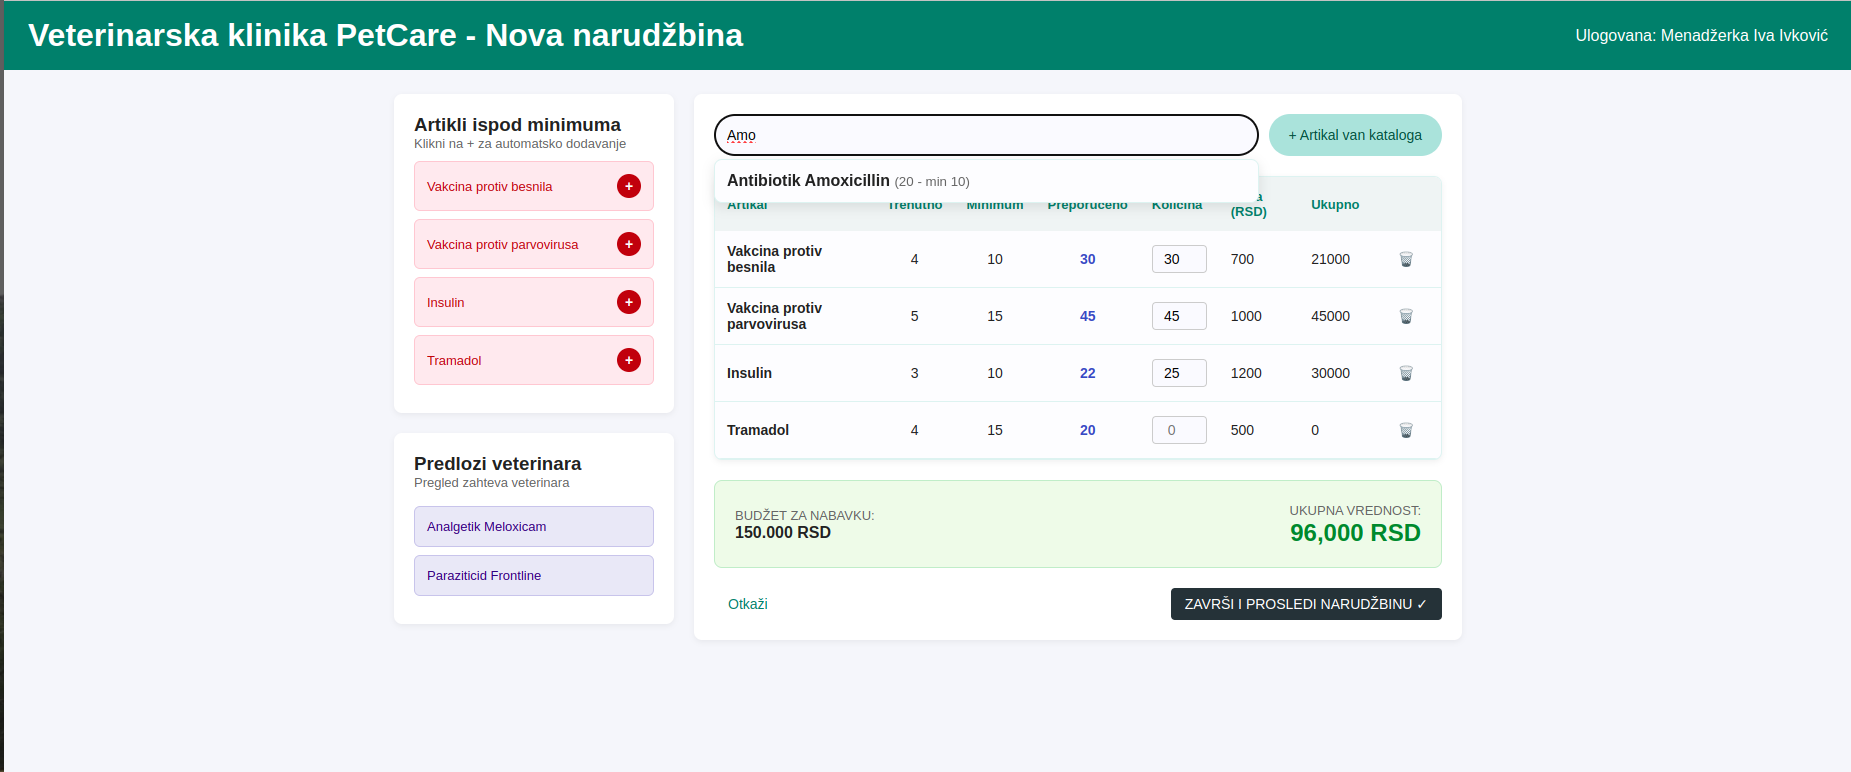
\includegraphics[scale = 0.18]{UI/Nova_narudzbina_3.png}
        \end{center}
    \end{figure}   
\end{frame}

\begin{frame}{Nova narudžbina}
        \begin{figure}[h!]
        \begin{center}
          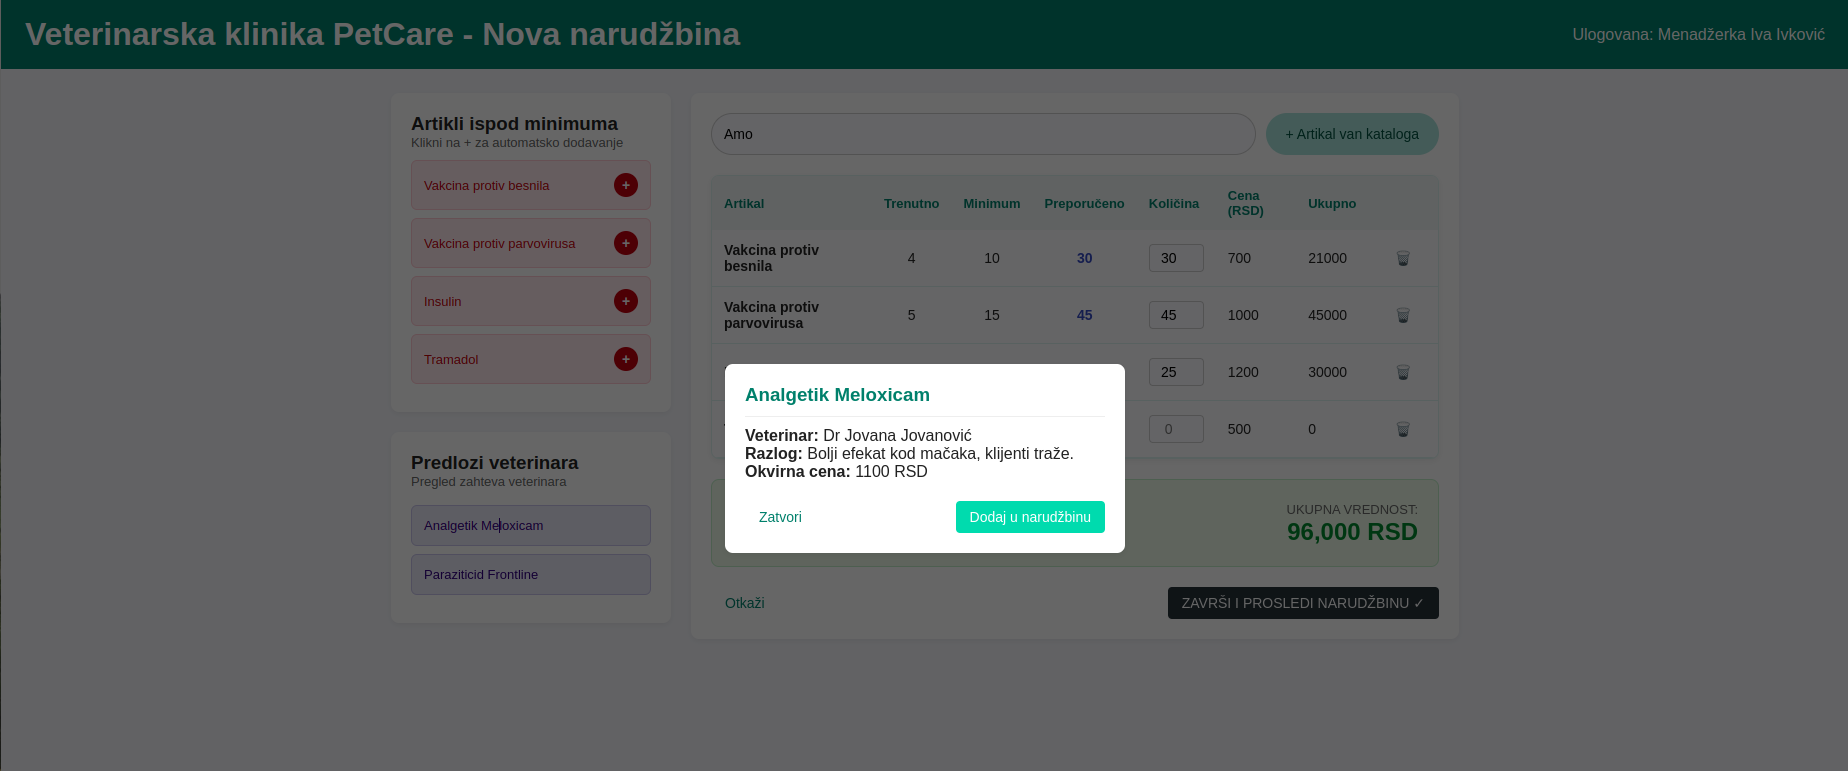
\includegraphics[scale = 0.18]{UI/Nova_narudzbina_4.png}
        \end{center}
    \end{figure}   
\end{frame}

\begin{frame}{Prijem robe}
        \begin{figure}[h!]
        \begin{center}
          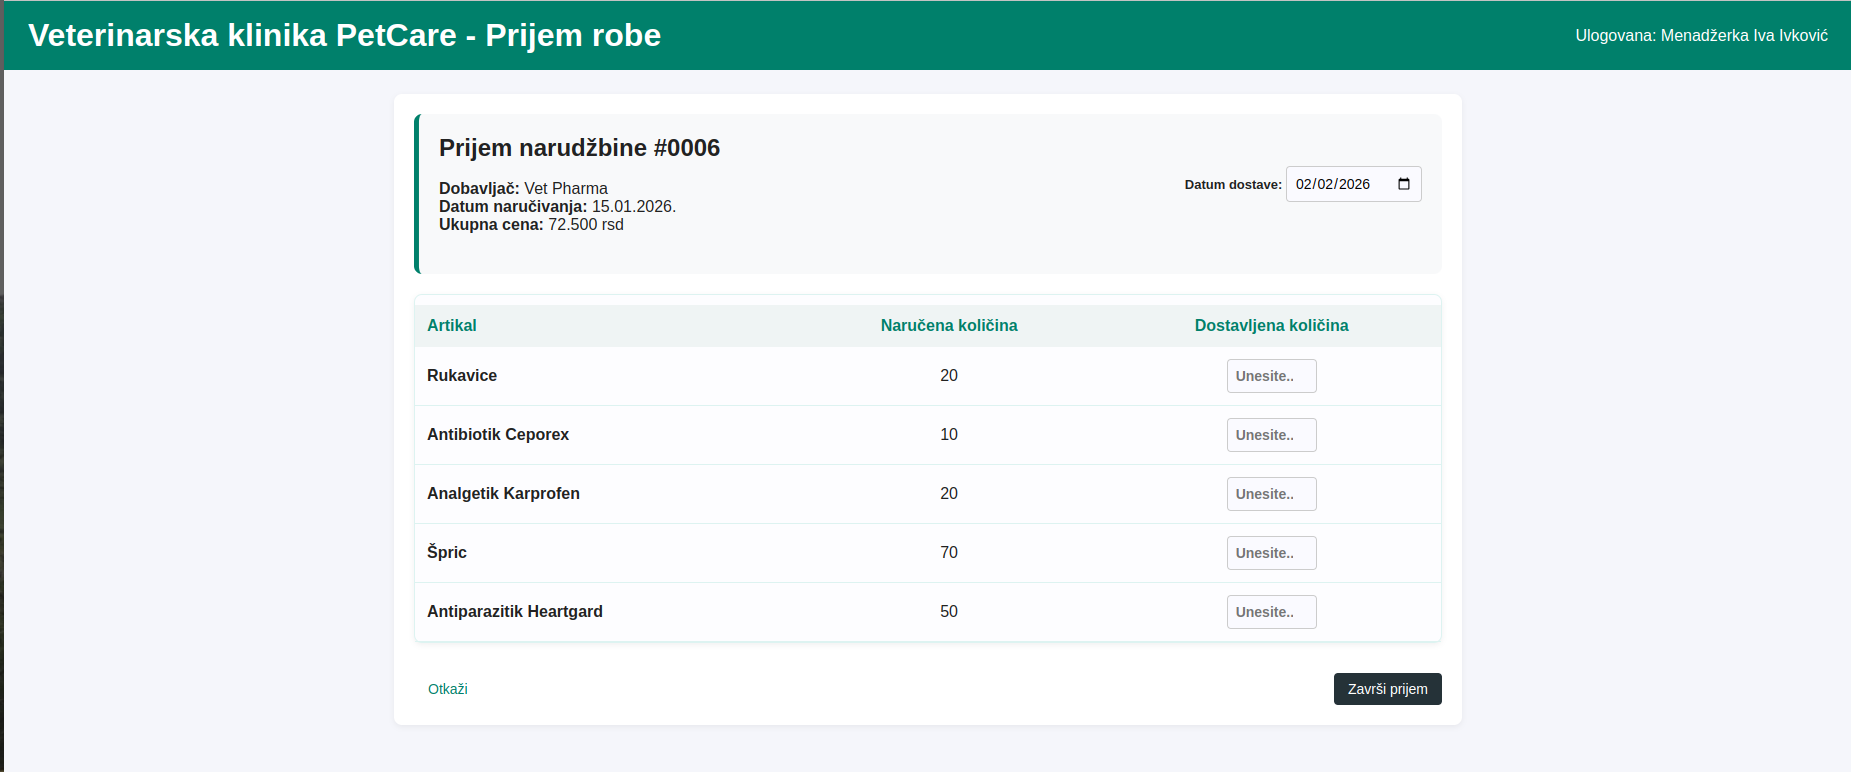
\includegraphics[scale = 0.18]{UI/Prijem_1.png}
        \end{center}
    \end{figure}   
\end{frame}

\begin{frame}{Prijem robe}
        \begin{figure}[h!]
        \begin{center}
          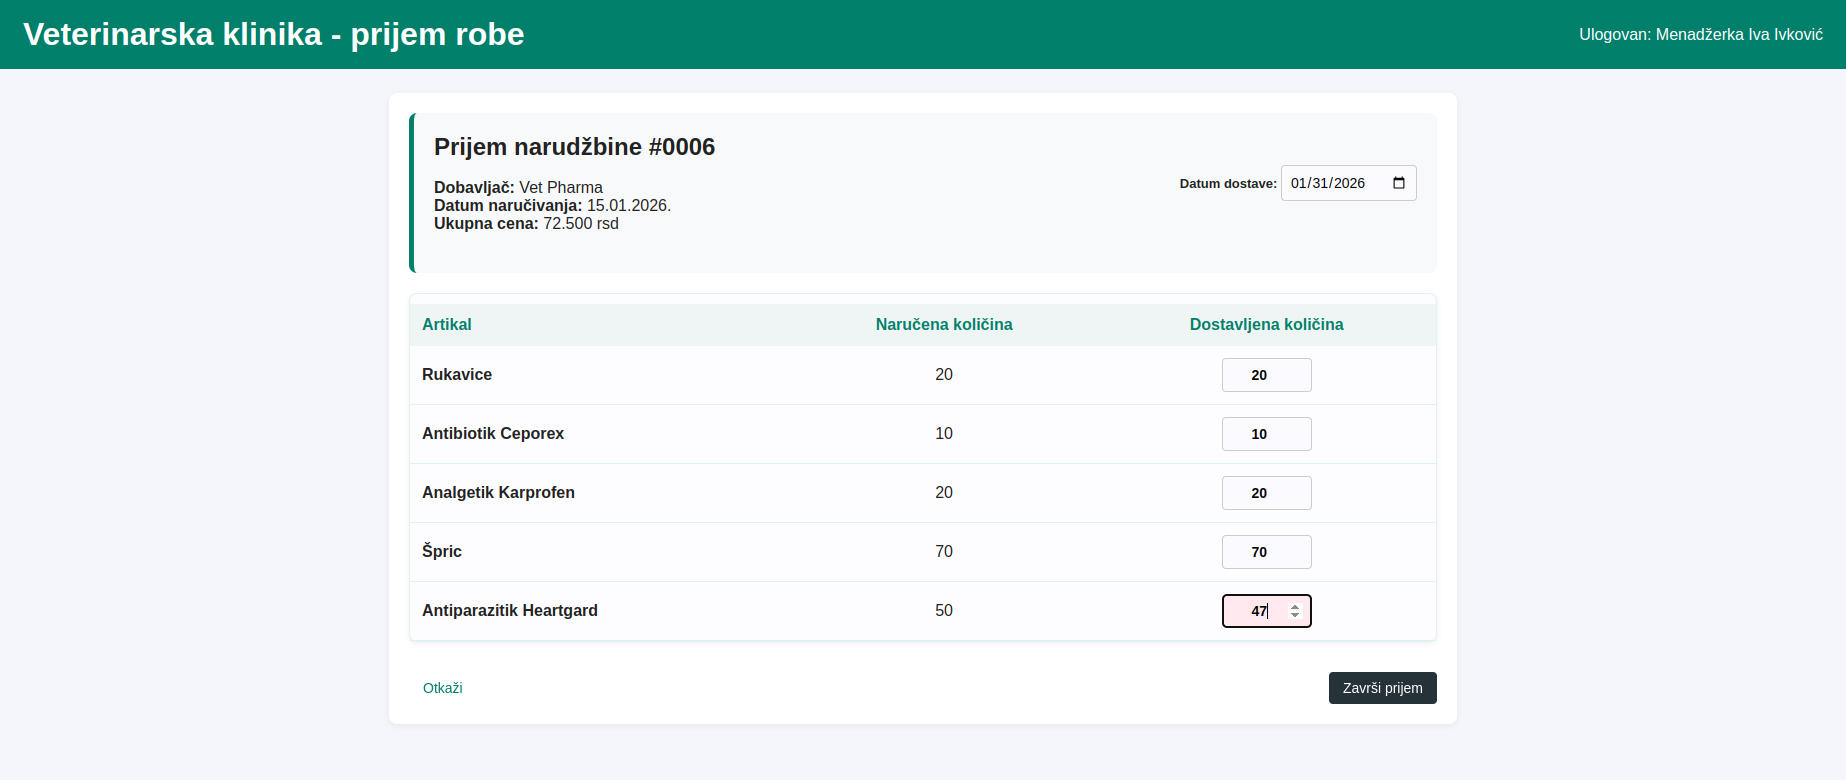
\includegraphics[scale = 0.18]{UI/Prijem_2.png}
        \end{center}
    \end{figure}   
\end{frame}


\begin{frame}{Prijem robe}
        \begin{figure}[h!]
        \begin{center}
          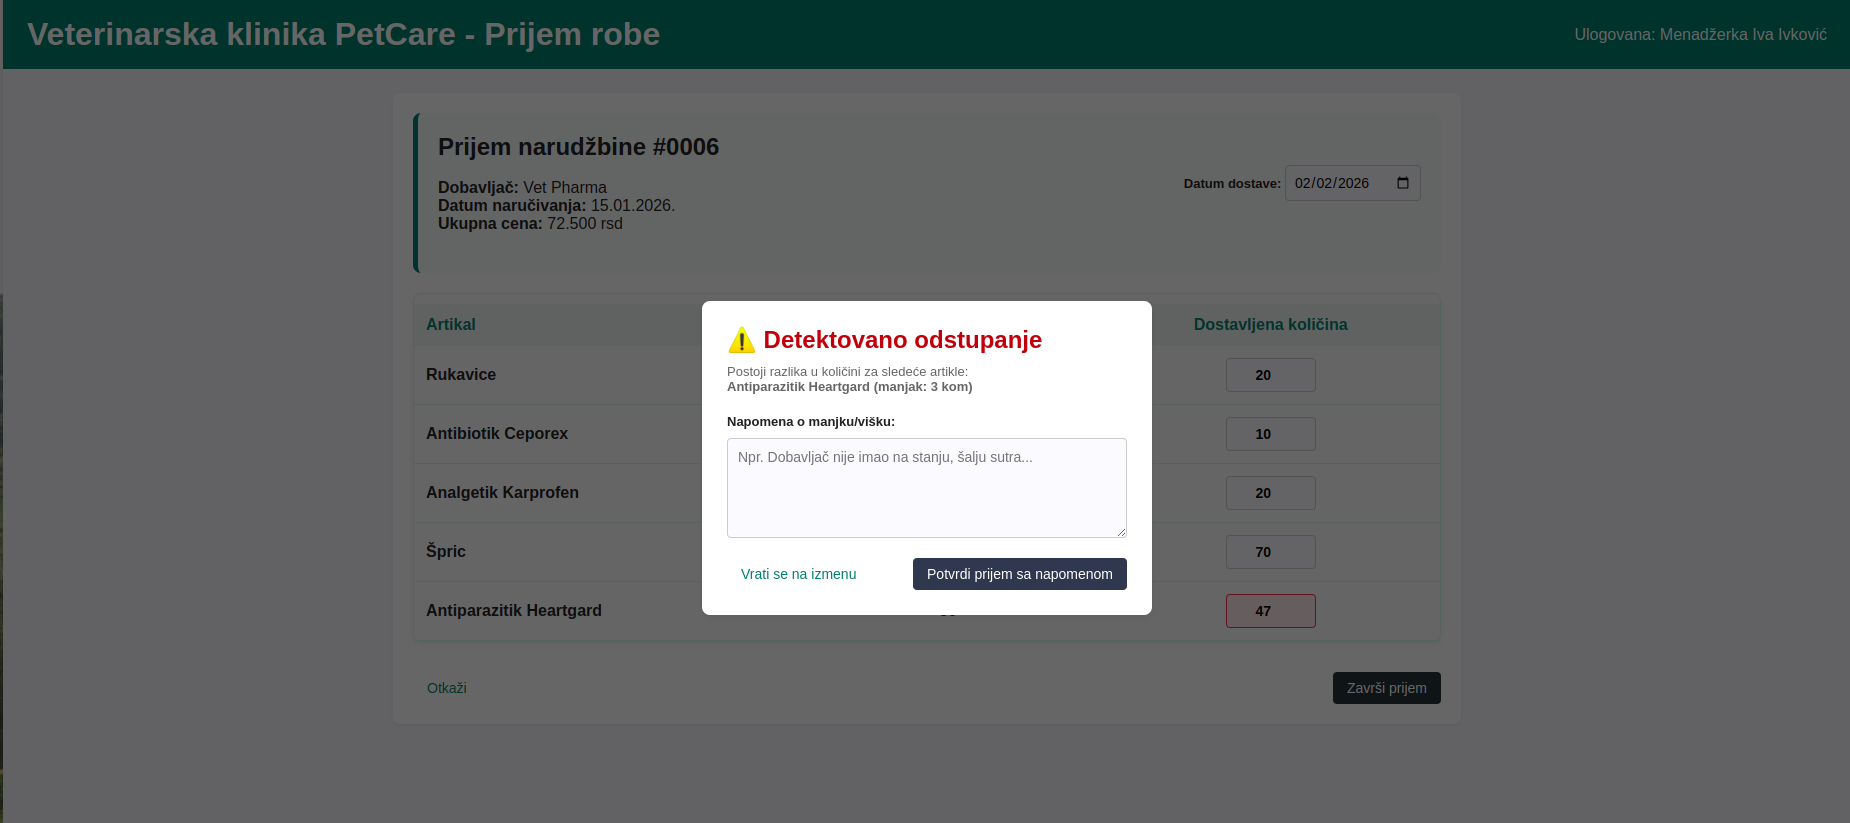
\includegraphics[scale = 0.18]{UI/Prijem_3.png}
        \end{center}
    \end{figure}   
\end{frame}


\begin{frame}{Zaključak}
\begin{itemize}
    \item U opisanom informacionom sistemu ističe se važnost komunikacije između inženjera/ki sa licima stručnim u oblasti za koju se kreira sistem - u našem slučaju je to veterinarska medicina i koliko ta komunikacija može uticati na tehnička rešenja. 
    \pause
    \item Funkcionalan sistem, takođe, mora da prati zakonske propise, posebno u oblasti zaštite ličnih i medicinskih podataka.
    \pause
    \item Samo uz razumevanje struke za koju se sistem kreira, poznavanja zakona i principa bezbednosti podataka moguće je razviti rešenje koje zaista unapređuje rad klinike i kvalitet pruženih usluga.
\end{itemize}
\end{frame}

\begin{frame}
    \vfill
    \centering
    \Huge Hvala na pažnji!
    \vfill
\end{frame}











\end{document}
